\chapter{Integration of Data Streams}\label{ch:int_data}
One rapidly emerging trend in the field of exoplanet studies is the application of multiple instruments and observatories to the study of a single target.  After the initial discovery of planets about HR8799 in data collected at the Keck and Gemini observatories \citep{marois2008direct}, evidence for these planets was also uncovered in archival Hubble Space Telescope (HST) data \citep{lafreniere2009hst} and multiple other groups have made followup observations at a variety of other observatories \citep{hinz2010thermal,janson2010spatially}.   Planetary candidates derived from Kepler Observations are all followed up with ground-based spectroscopic and photometric studies before they can be confirmed as new planets \citep{borucki2010kepler,borucki2011characteristics}.  Similarly, proposed planet-finding instruments using astrometric techniques usually assume a pre-existing (or concurrently collected) radial velocity data set to help with orbit fitting \citep{catanzarite2006}.  This trend points to the importance of developing systematic ways of combining disparate data sets of the same target stars into unified exosystem models.  This chapter will describe one such method, drawing heavily on the modeling work developed throughout this thesis.

\section{Exosystems as Hidden Markov Models}\label{sec:hmm}
Regardless of how we observe an exosystem, we are making measurements of an underlying system with deterministic dynamics.  If we had sufficient information about all of the bodies in the exosystem (e.g., equal to the amount of data we have about our own solar system), then we could predict the positions and photometric properties of all of the bodies in that system far into the future.  Unfortunately, our observation methods give us only brief snapshots of small portions of exosystem dynamics, so that we have to reconstruct the full picture from multiple observations and modeling.  It is this property of planet-finding that makes Hidden Markov Models (HMM), Dynamic Bayesian Networks (DBN) and dynamic filtering so appropriate to describing exoplanet observations.

We assume a dynamic system with state variable $X_t$ whose evolution in time is a Markov process, i.e.:
\begin{equation}
\begin{split}
P[X_k = x_k | X_{k-1} = x_{k-1}, X_{k-2} = x_{k-2}, X_{k-3} = x_{k-3}, \ldots]\\
 = P[X_k = x_k | X_{k-1} = x_{k-1}] \,.
 \end{split}
\end{equation}
An HMM is generated when some part of the state is unobserved.  If our knowledge of the system comes from observations:
\begin{equation}
Y_t = f(X_t)
\end{equation}
the state is partially observed when function $f$ discards some portion of $X_t$.  For example, if $X_t \in \mathbb R^n$, then the state is partially observed when $f: \mathbb R^n \rightarrow \mathbb R^m$ for $m < n$. A generalization of this formalism yields dynamic Bayesian networks, where the system evolution is governed by temporal probability models, and leads us to the idea of dynamic filtering and state estimation \citep{russell1995artificial}.

In general, if we know how $X_t$ evolves in time and how $Y_t$ depends on $X_t$, via either probabilities or flows, we can use time histories of observations to approximate the time history (and current value) of the state.  More specifically, for a Markov process with state $\mf x$ and observation $\mf z$:
\begin{equation}
P\left[\mf x_0,\mf x_1\ldots \mf x_n, \mf z_1,\mf z_2 \ldots \mf z_n\right] = P\left[\mf x_0\right] \prod_{j = 1}^{n} P\left[\mf z_j | \mf x_j\right]P\left[\mf x_j | \mf x_{j-1}\right] \,,
\end{equation}
the next state can be predicted from the observed history as:
\begin{equation} \label{eq:bayesPredict}
P\left[\mf x_j | \mf z_{1:j-1}\right] = \int_{\mf x_{j-1}} P\left[\mf x_j | \mf x_{j-1}\right]P\left[\mf x_{j-1} | \mf z_{1:j-1}\right] \intd{\mf x_{j-1}} \footnote{The subscript $1:j-1$ represents the joint distribution $\mf z_1, \mf z_2, \mf z_3, \ldots \mf z_{j-1}$} \,,
\end{equation}
and updated with the current observation via Bayes rule:
\begin{equation}\label{eq:bayesUpdate}
P\left[\mf x_j|\mf z_{1:j}\right] = \frac{P\left[\mf z_j | \mf x_j\right] P\left[\mf x_j | \mf z_{1:j-1}\right[}{P\left[\mf z_j | \mf z_{1:j-1}\right]} \,.
\end{equation}

Alternatively, we can write the state update and observation as functions with additive noise terms:
\begin{align}
\mf x_{k+1}& = \mf f(\mf x_k,k) + \bf w_k \label{eq:stateUpdate}\\
\mf z_k &= \mf h(\mf x_k,k) + \bf n_k \label{eq:observation}
\end{align}
where $\bf w_k$ and $\bf n_k$ are the process noise and measurement noise, respectively.  Note that while Equations (\ref{eq:stateUpdate}) and (\ref{eq:observation}) represent discrete time systems, an equivalent formalism exists for continuous time systems of the form:
\begin{align}
\frac{\mathrm{d}\mf x(t)}{\mathrm{d}t}  &= \mf f(\mf x(t),t) + \bf w(t) \label{eq:stateUpdateCont}\\
\mf z(t) &= \mf h(\mf x(t),t) + \bf n(t) \label{eq:observationCont} \,.
\end{align}
In this formulation, we can define a state estimate, $\hat{\mf x}$, that is optimal in some sense---for example minimizing mean-square error:
\begin{equation}
\hat{\mf x}_k = \arg\min E\{\Vert \mf x_k - \hat{\mf x}_k\Vert^2\} \,,
\end{equation}
in which case the state estimate for a time history of $N$ observations corresponds to the minimization (with respect to $\mf x$) of the quadratic cost function:
\begin{equation} \label{eq:filteringCost}
J = \sum_{k=1}^N \left[\mf z_k - \mf f(\mf x_k,k) \right]^T R^{-1}\left[\mf z_k -\mf f(\mf x_k,k) \right]
\end{equation}
where $R$ is a weighting matrix often taken to be the observation noise covariance.  In many cases \refeq{eq:filteringCost} represents a non-convex optimization problem and is more tractable when formulated as a recursive filter \citep{crassidis2004}.

As in Equations (\ref{eq:bayesPredict}) and (\ref{eq:bayesUpdate}) the recursive filter predicts the next state based on the current state and the system dynamics ($\mf f$), and then updates this prediction by incorporating the next measurement and taking into account the spectral density of the measurement noise.  The most well known of these filters is the Kalman filter, which assumes zero-mean, white, Gaussian process and measurement noise, and can be shown to be optimal (in the minimum least-squares error sense) for linear state and observation equations; i.e., where $\mf f $ and $\mf h$ can be written as:
\begin{align}
\mf f(\mf x_k,k) &= \mf F_k \mf x_k \label{eq:linStateUpdate}\\
\mf h(\mf x_k,k) &= \mf H_k \mf x_k \,.
\end{align}
The Kalman filter has been successfully applied to a wide range of problems including navigation and tracking systems, computer vision, and radio and telecommunications systems \citep{stengel1994optimal,crassidis2004}.  There is also an extensive body of literature on using Kalman filters for orbit and attitude estimation (see, for example \citet{spilker1996global}).

The Kalman filter can be though of as estimating the change in the distribution function of the state by propagating its first two central moments: the mean and variance.  This operation is greatly simplified by noting that if the current distribution of a state is Gaussian then the predicted state distribution using a linear Gaussian transition model $P\left[\mf x_j | \mf x_{j-1}\right]$ (as in \refeq{eq:bayesPredict}) will also be a Gaussian distribution.  Similarly, if the observation model $P(\mf z_j | \mf x_j)$ is also linear Gaussian then the updated state distribution will be Gaussian as well.  This makes it relatively simple to propagate linear Gaussian state distributions in time, as long as the initial conditions correspond to the true distribution.

For a linear state update (as in \refeq{eq:linStateUpdate}) the predicted state estimate $\hat{\mf x}_k$ given the previous estimate $\hat{\mf x}_{k-1}$ is: 
\begin{equation}
\hat{\mf x}_{k|k-1} =  \mf F_k \hat{\mf x}_{k-1|k-1} \,.
\footnote{The notation used here represents the predicted (\emph{a priori}) values via the subscript $k|k-1$ and the updated (\emph{a posteriori}) values via the subscript $k|k$.  An alternate convention (c.f., \citet{stengel1994optimal}) is to label predicted values with a minus sign ($\hat{\mf x}_k(-)$ or $\hat{\mf x}_k^-$) and updated values with a plus sign  ($\hat{\mf x}_k(+)$ or $\hat{\mf x}_k^+$).} 
\end{equation}
From this, we find that the state covariance, defined as:
\begin{equation}
\mf P_k = E[(\mf x_k - E[{\mf x}_k])(\mf x_k - E[{\mf x}_k])^T] \,,
\end{equation}
is predicted as:
\begin{equation}
\mf P_{k|k-1} =  \mf F_k \hat{\mf x}_{k-1|k-1} \mf F_k^T + \mf Q_k \,,
\end{equation}
where $\mf Q_k$ is the covariance of the process noise:
\begin{equation}
\mf w_k \sim N(0,\mf Q_k) \,.
\end{equation}
If the initial state estimate and covariance accurately reflect the state distribution:
\begin{equation}\label{eq:KalmanICs}
\begin{split}
\hat{\mf x}_0 &= E[\mf x_0]\\
\mf P_0 &= E[(\mf x_0 - \hat{\mf x}_0)(\mf x_0 - \hat{\mf x}_0)^T]
\end{split}
\end{equation}
then all subsequent state estimates  should have zero mean error:
\begin{equation}
E[\mf x_k - \hat{\mf x}_k] = 0 \,.
\end{equation}
This is achieved by updating the predicted state with the current measurement as:
\begin{equation}
\hat{\mf x}_{k|k} = \hat{\mf x}_{k|k-1} + \mf K_k \left( \mf z_k - \mf H_k \hat{\mf x}_{k|k-1}\right)\,,
\end{equation}
where $\mf K_k$ is the optimal Kalman gain that minimizes the updated estimate mean square error, $E[(\mf x_k - \hat{\mf x}_{k|k})^T(\mf x_k - \hat{\mf x}_{k|k})]$, and has the form:
\begin{equation}\label{eq:KalmanGain}
\mf K_k = \mf P_{k|k-1} \mf H_k^T \left(\mf H_k \mf P_{k|k-1} \mf H_k^T + \mf R_k\right)^{-1} \,,
\end{equation}
where $\mf R_k$ is the covariance of the observation noise:
\begin{equation}
\mf n_k \sim N(0,\mf R_k) \,.
\end{equation}
\refeq{eq:KalmanGain} can be derived in a variety of ways, the simplest of which is to write the cost function in \refeq{eq:filteringCost} for two subsequent measurements, substituting $\mf H_k \hat{\mf x}_k$ for $\mf f(\mf x_k,k)$, and to then minimize the resulting function.  This then allows us to write the updated covariance as:
\begin{equation} \label{eq:covUpdate}
\mf P_{k|k} = \left(\mf P_{k|k-1}^{-1} + \mf H_k^T \mf R_k^{-1} \mf H_k \right)^{-1} \,.
\end{equation}
Alternatively, we can take advantage of the fact that minimizing the mean-square error is equivalent to minimizing the trace of the updated covariance, which leads to the equivalent Kalman gain expression, but requires us to first define $\mf P_{k|k}$.  This is done by noting that the updated covariance must equal the covariance of the error:
\begin{align}
\mf P_{k|k} &= E\left[\left((\mf x_k - \hat{\mf x}_{k|k}) - E[(\mf x_k - \hat{\mf x}_{k|k})]\right)\left((\mf x_k - \hat{\mf x}_{k|k}) - E[(\mf x_k - \hat{\mf x}_{k|k})]\right)^T\right] \\
&= \left(I - \mf K_k \mf H_k\right) \mf P_{k|k-1} \left(I - \mf K_k \mf H_k\right)^T + \mf K_k \mf R_k \mf K_k^T\,,
\end{align}
where $I$ is the identity matrix.
When $\mf K_k$ has the form in \refeq{eq:KalmanGain}, this further simplifies to:
\begin{equation}
\mf P_{k|k} = \left(I - \mf K_k \mf H_k\right) \mf P_{k|k-1} \,,
\end{equation}
which can be shown to be equivalent to \refeq{eq:covUpdate} via the matrix inversion lemma \citep{stengel1994optimal}.


The Kalman-Bucy filter extends this formalism to continuous time systems, as in Equations (\ref{eq:stateUpdateCont}) and (\ref{eq:observationCont}), where again $\mf f$ and $\mf h$ are linear in $\mf x$ (but possibly time varying):
\begin{align}
\mf f(\mf x(t),t) &= \mf F(t) \mf x(t) \label{eq:linStateUpdateCont}\\
\mf h(\mf x(t),t) &= \mf H(t) \mf x(t) \,.
\end{align}
The resulting filter is defined via the differential equations:
\begin{align}
\frac{\mathrm{d}\hat{\mf x}(t)}{\mathrm{d}t} &= \mf F(t)\hat{\mf x}(t) + \mf K(t) \left( \mf z(t) - \mf H(t) \hat{\mf x}(t)\right) \\
\frac{\mathrm{d}\mf P(t)}{\mathrm{d}t} &=  \mf F(t)\mf P(t) + \mf P(t) \mf F^T(t) + \mf Q(t) -  \mf K(t) \mf R(t) \mf K^T(t) \\
\mf K(t) &= \mf P(t) \mf H^T(t) \mf R^{-1}(t) \,.
\end{align}
Most physical system, including those studied here, are not actually observed continuously, so that the fully continuous Kalman-Bucy equations are not particularly helpful.  However, it is possible to write a hybrid filter for the system:
\begin{align}
\frac{\mathrm{d}\mf x(t)}{\mathrm{d}t}  &= \mf F(t) \mf x(t) + \mf w(t) \\
\mf z_k &= \mf H_k\mf x(t_k) + \mf v_k \,,
\end{align}
where $t_k$ is an element of the set of observation times $\{t_i\}$.  The resulting hybrid equations are then:
\begin{align}
\hat{\mf x}_{k|k-1} &= \int_{t_{k-1}}^{t_k} \mf F(t)\hat{\mf x}(t) \intd{t} \label{eq:hybridKalmanStatePredict}\\
\mf P_{k|k-1} &=  \int_{t_{k-1}}^{t_k}  \mf F(t)\mf P(t) + \mf P(t) \mf F^T(t) + \mf Q(t) \intd{t} \label{eq:hybridKalmanCovPredict} \\
\mf K_k &= \mf P_{k|k-1} \mf H_k^T \left(\mf H_k \mf P_{k|k-1} \mf H_k^T + \mf R_k\right)^{-1}  \\
\hat{\mf x}_{k|k} &= \hat{\mf x}_{k|k-1} + \mf K_k \left( \mf z_k - \mf H_k \hat{\mf x}_{k|k-1}\right) \\
\mf P_{k|k} &= \left(\mf P_{k|k-1}^{-1} + \mf H_k^T \mf R_k^{-1} \mf H_k \right)^{-1} \label{eq:hybridKalmanCovUpdate} \,,
\end{align}
with the state and covariance initialized as in \refeq{eq:KalmanICs} and $\hat{\mf x}_{k-1|k-1}$ and $\mf P_{k-1|k-1}$ used as the initial conditions for the integrations in Equations (\ref{eq:hybridKalmanStatePredict}) and (\ref{eq:hybridKalmanCovPredict}), respectively.


When the state and measurement equations are nonlinear, the Kalman formalism can still be applied to the linearized system, yielding the Extended Kalman Filter (EKF).  Unlike the original Kalman filter, the extended filter is no longer guaranteed to be an optimal estimator, and can produce highly divergent estimates in cases where the filter pushes the state outside the neighborhood of the linearization \citep{crassidis2004}.  Nevertheless, the EKF is widely applied and can produce good results with comparatively small computational costs.  The equations for the hybrid EKF are the same as (\ref{eq:hybridKalmanStatePredict}) - (\ref{eq:hybridKalmanCovUpdate}), except that $\mf F$ and $\mf H$ are now the linearizations of $\mf f$ and $\mf h$:
\begin{align}
\mf F(t) &= \left.\frac{\partial \mf f(\mf x(t),t)}{\partial \mf x}\right|_{\hat{\mf x}(t)} \\
\mf H_k &= \left.\frac{\partial \mf h(\mf x(t),t)}{\partial \mf x} \right|_{\hat{\mf x}_{k|k-1}}
\end{align}
and the state update equation uses the nonlinear measurement:
\begin{equation}\label{eq:hybridEKFStateUpdate}
\hat{\mf x}_{k|k} = \hat{\mf x}_{k|k-1} + \mf K_k \left( \mf z_k - \mf h(\hat{\mf x}_{k|k-1},t_k)\right) \,.
\end{equation}
A sample implementation of the hybrid EKF is presented in \refcode{code:hybridEKF}.  

Because the linearization of the system dynamics makes $\mf F(t)$ a function of $\hat{\mf x}(t)$, the differential equations  (\ref{eq:hybridKalmanStatePredict}) and (\ref{eq:hybridKalmanCovPredict}) must be integrated simultaneously as a single system:
\begin{equation}\label{eq:stateCovIntegration}
\begin{bmatrix} \hat{\mf x}_{k|k-1} \\\ \mf P_{k|k-1} \end{bmatrix} = 
\int\limits_{t_{k-1}}^{t_k} \begin{bmatrix}  \mf F(t)\hat{\mf x}(t) \\\   \mf F(t)\mf P(t) + \mf P(t) \mf F^T(t) + \mf Q(t) \end{bmatrix} \intd{t} \,.
\end{equation}
To deal with the nonlinearities introduced by nonlinear observation equations, it is common to iterate the state update equations as:
\begin{align}
\mf H_{k_i} &= \left.\frac{\partial \mf h(\mf x(t),t)}{\partial \mf x} \right|_{\hat{\mf x}_{k|{k_i}}} \\
\mf K_{k_i} &= \mf P_{k|k-1} \mf H_{k_i}^T \left(\mf H_{k_i} \mf P_{k|k-1} \mf H_{k_i}^T + \mf R_k\right)^{-1}  \\
\hat{\mf x}_{k|{k_i}} &= \hat{\mf x}_{k|k-1} + \mf K_{k_i} \left( \mf z_k - \mf h(\hat{\mf x}_{k|{k_{i-1}}},t_k)
- \mf H_{k_i}\left( \hat{\mf x}_{k|k-1} -  \hat{\mf x}_{k|{k_{i-1}}} \right)\right) \,
\end{align}
where the iteration is initialized with $\hat{\mf x}_{k|{k_0}} = \hat{\mf x}_{k|k-1}$ and run until
\begin{equation}
\max \left\vert \hat{\mf x}_{k|{k_{f}}}  - \hat{\mf x}_{k|{k_{f-1}}} \right\vert \le \epsilon 
\end{equation}
for desired convergence level ($\epsilon$).  The covariance update is then calculated from $\hat{\mf x}_{k|{k_{f}}}$ using \refeq{eq:hybridKalmanCovUpdate} with $\mf H_{k_f}$.  

Another modification that can be made is the introduction of constraints to the state.  If the chosen state for a nonlinear system can describe physically impossible (or undesirable) configurations, then it makes sense to constrain the state at each filter iteration.  For example, if we use position and velocity to describe planetary orbits, our state can describe open (hyperbolic) orbits just as easily as closed ones.  Since it is highly unlikely that we will find any exoplanet on an escape trajectory from its parent star, we may wish to constrain the Keplerian orbital energy of the orbits described by our state vector to be negative or zero at each time step.  

Following \citet{simon2006}, we introduce a set of inequality constraints of the form:
\begin{equation}
D \mf x \le \mf d
\end{equation}
where $D$ is a known $m \times n$ matrix (for $m$ constraints of $n$ state variables, such that $m \le n$), and $\mf d$ is the vector of constraints.  The filter state can then be constrained by introducing a quadratic programming problem into the filter iteration of the form:
\begin{equation}
 \min_{\tilde{\mf x}} \left(\tilde{\mf x}^TW\tilde{\mf x} - 2 \hat{\mf x}_{k|k}^TW\tilde{\mf x} \right) \quad\textrm{such that}\quad D \tilde{\mf x} \le \mf d
\end{equation}
where $\tilde{\mf x}$ is the constrained state estimate and $W$ is a symmetric positive definite matrix.  The solution to this problem is equivalent to the solution of the equivalent equality constraint problem \citep{simon2002kalman}, and is given by:
\begin{equation} \label{eq:ineqConstraintSol}
\tilde{\mf x} =  \hat{\mf x}_{k|k} - W^{-1}D^T\left(D W^{-1}D^T\right)^{-1}\left(D \hat{\mf x}_{k|k} - \mf d\right) \,.
\end{equation}

 Selecting $W = \mf P_{k|k}^{-1}$ has the effect of maximizing the conditional probability $P(\tilde{\mf x} | \mf z_k)$.  Alternatively, taking $W$ to be the identity matrix is equivalent to minimizing the conditional mean square error:
\begin{equation}
E\left[\Vert  \mf x_{k|k} - \tilde{\mf x} \Vert^2 | \mf z_k \right] \,.
\end{equation}
In either case, using \refeq{eq:ineqConstraintSol} we can write the expected value of the constrained estimate error as:
\begin{equation}
E\left[\mf x - \tilde{\mf x}\right] = \left(I - W^{-1}D^T\left(D W^{-1}D^T\right)^{-1}D\right)E\left[\mf x - \hat{\mf x}_{k|k}\right]  \,,
\end{equation}
and since the expected value of the error associated with the Kalman filter state estimate is zero, so is the expected value of the constrained estimate error.  Thus, the constrained state estimate is an unbiased estimator for the system, just like the original unconstrained state estimate \citep{simon2006}.

Because all of the equations used to formulate the filter are time reversible, every Kalman filter can also be used as a smoother, i.e., to find the most probable values of a state at some time $t$ where $t_0 < t < t_f$ while using the whole data set from $t_0$ to $t_f$.  The only exception to this generalization is if the numerical integrator used in the EKF is not time reversible, which holds true for a class of symplectic integrators \citep{yoshida1993recent}, but is not an issue for the methods used here.  It is common to perform multiple smoothing and filtering steps on noisy data although for nonlinear systems, there is no guarantee that the state estimates will ever converge to some final values.

There are also many other variations, refinements and extensions of the Kalman filter.  One family of filters, called Unscented Kalman Filters (UKF), first introduced in \citet{julier1995new}, seeks to improve upon the EKF by taking into account the second order terms in the expansion of the system dynamics, thereby increasing the probability that the propagated state distribution remains in the neighborhood of the linearization.  	This is done by propagating a minimal set of points of the same mean and covariance as the state distribution and calculating the updated state and covariance estimates from their updated values.  The set is selected so that the distribution can be modeled to second order accuracy with 2$n$ points \citep{julier1995new,julier2004unscented,van2001square}.  

More specifically, for an $n$-dimensional (Gaussian) distribution of states, given a state mean and covariance estimate, we generate a set of points (often called `sigma' points):
\begin{align}
\chi_0 &= \hat{\mf x}_{k|k}\\
\left\{\chi_{k|k}^i\right\}_{i=1}^{2n} &= \hat{\mf x}_{k|k} \pm \textrm{col}\left[ \sqrt{(n+\lambda) \mf P_{k|k}}\right], 
\end{align}
where col represents the column operator (which equals the set of columns of the argument matrix) and the square root of the scaled covariance can be found using the Cholesky decomposition.  The scaling parameter $\lambda$ is defined via positive constant parameters $\alpha$ and $\gamma$ such that:
\begin{equation}
\gamma = \alpha^2(n  + \lambda) - n\,.
\end{equation}

The sigma points are propagated via the system dynamics:
\begin{equation}
\chi_{k|k-1}^i = \mf f(\chi_{k-1|k-1}^i,k) \,,
\end{equation}
and the predicted mean and covariance are computed as:
\begin{align}
\hat{\mf x}_{k|k-1} &= \sum_{i=0}^{2n} W_m^i \chi_{k|k-1}^i \\
\mf P_{k|k-1} &= \sum_{i=0}^{2n} W_c^i \left(\chi_{k|k-1}^i - \hat{\mf x}_{k|k-1}\right) \left(\chi_{k|k-1}^i - \hat{\mf x}_{k|k-1}\right)^T  + \mf Q_k\,,
\end{align}
where $\{W_m\}$ and $\{W_c\}$ are weight sets defined as:
\begin{align}
W_m^i &= \begin{cases} \frac{\gamma}{n+\gamma} & i = 0\\ \frac{1}{2(n+\gamma)} & \textrm{else}\end{cases} \\
W_c^i &= \begin{cases} \frac{\gamma}{(n+\gamma) + (1 - \alpha^2 + \beta)} & i = 0\\  \frac{1}{2(n+\gamma)} & \textrm{else} \end{cases}
\end{align}
with:
\begin{equation}
\kappa = \alpha^2(n  + \lambda) - n
\end{equation}
for positive constants $\beta$.
A new set of sigma points $\left\{\chi_{k|k}^i\right\}$ is generated from the predicted covariance $\mf P_{k|k-1}$ and the predicted observations are calculated from the observation equation:
\begin{equation}
\zeta_k^i = \mf h(\chi_{k|k}^i,k) \,.
\end{equation}
The Kalman gain can then be calculated as:
\begin{equation}
\mf K_k = \left(\sum_{i=0}^{2n} \left(\chi_{k|k}^i - \sum_{j=0}^{2n} W_m^j \chi_{k|k-1}^j \right) W_c^i\left(\zeta_k^i -  \sum_{j=0}^{2n} W_m^j \zeta_{k}^j \right)^T \right)\mf S_k^{-1}
\end{equation}
where
\begin{equation}
\mf S_k = \sum_{i=0}^{2n} \left(\zeta_k^i -  \sum_{j=0}^{2n} W_m^j \zeta_{k}^j \right) W_c^i\left(\zeta_k^i -  \sum_{j=0}^{2n} W_m^j \zeta_{k}^j \right)^T  - \mf R_k \,,
\end{equation}
so that the state and covariance updates become:
\begin{align}
\hat{\mf x}_{k|k} &= \hat{\mf x}_{k|k-1} + \mf K_k\left(\mf z_k -  \sum_{i=0}^{2n} W_m^i \zeta_k^i\right) \\
\mf P_{k|k} &= \mf P_{k|k-1} - \mf K_k\mf S_k\mf K_k^T\,.
\end{align}

The literature varies in the particular values to be used for the various constant parameters.  \citet{van2001square} suggest that $\alpha$ (which determines the spread of the sigma points about the state esimtate) be taken from the range of $(1\times10^{-4}, 1)$, $\beta$ (which determines how much prior knowledge of the state distribution should be incorporated) should be equal to 2 for Gaussian distributions, and that $\lambda$ should be set to zero for state estimation and $n - 3$ for parameter estimation.  The optimal values for a given system are often determined via empirical checks, rather than being derived rigorously from first principles.  As with the EKF, the UKF can be extended to continuous time systems and hybrid systems \citep{sarkka2007unscented}.  A sample implementation of a hybrid UKF is presented in \refcode{code:hybridUKF}.

In addition to Kalman filters, there is also the family of particle filters, also known as sequential Monte Carlo (SMC) methods.  These also model the state distribution via a population of points, but use much larger sets in an attempt to capture the true state distribution.  This means that these filters can relax the assumptions of Gaussian noise at the cost of a significantly higher computational burden \citep{van2001unscented,ng2005continuous}. Another recent innovation on the UKF--- the $j$th moment extended Kalman filter (JMEKF) ---involves the propagation of higher order moments of the state distribution (instead of just the first two) and is described in \citet{majji2008high}.  This technique requires automated expansion of the system dynamics about the current state estimate and can be very computationally intensive.  The latest refinements of this filter include incorporation of perturbation techniques to derive the time evolution of the higher order moments of the estimation error \citep{majji2010perturbation}.  For the purposes of the analysis in this chapter, we assume that the process and observation noise are approximately Gaussian, and use the formalism of the EKF and UKF.  However, as advances are made in the efficient computation of the various higher order filters, it may prove useful to apply these as well.  The same descriptions of the state, system dynamics, and observation functions can be utilized, regardless of the specific filter update equations.

\section{Initializing the State}\label{sec:state_init}
\subsection{Selecting the State Vector}\label{sec:state_selection}
In order to apply the formalism developed in the previous section, it is first necessary to define the state that will be used to describe the exosystem.  The only requirements on this state are that it must be able to model the dynamics of the exosystem (i.e., the orbital motion) and that it must map to any observation method.  The simpler (and more linear) these mappings, the better.  In fact, we have already defined one such state when discussing the parameter sets necessary to encode simulated planetary systems in \S\ref{sec:gen_plan_sys}.  We can define a `dynamic' state from the parameters in \refeq{eq:simParamSet}:
\begin{equation}
\mf x_d = \begin{bmatrix} \mf r_{i/G} &  {}^\mc I \mf v_{i/G}& \mu_i \end{bmatrix}^T\,, \quad i \in X
\end{equation}
where $X$ is the set of all exosystem bodies (see \refeq{eq:Xsetdef}) and $G$ is the exosystem barycenter\footnote{While the ordering of the specific elements is fairly arbitrary, the equations in the previous section all assume that the state is a column vector. By default, we will stack the positions and velocities of each body in turn, followed by all the gravitational parameters, i.e.: $\mf x_d = \begin{bmatrix} \mf r_{1/G} & {}^\mc I \mf v_{1/G}& \mf r_{2/G} & {}^\mc I \mf v_{2/G}&\ldots  &\mu_1 & \mu_2 &\ldots \end{bmatrix}^T$.}.  As discussed in \S\ref{sec:exosystem_params} and \S\ref{sec:sysProp}, one instance of the elements of $\mf x_d$ is sufficient to propagate the orbits of the exosystem indefinitely both forwards and backwards in time.

As shown in \refch{ch:obs_methods}, $\mf x_d$ can be mapped to a variety of observation methods, as long as we incorporate a few additional constant parameters:
\begin{equation}
\mf x_c = \begin{bmatrix} p_j & R_i & \mf r_\mu& \varpi \end{bmatrix}^T\,, \quad j \in Y
\end{equation}
where $Y$ is the set of all exosystem bodies excluding the star (see \refeq{eq:keplerCOM}).  We can also include the planets' effective temperatures, if we are interested in detailed modeling of the spectra, or using spectral information to improve orbital fits \citep{barman2001irradiated, hauschildt2008irradiated, burrows2003beyond}.  Our final state is the combination of the static and dynamic states:
\begin{equation}\label{eq:stateVector}
\mf x = \begin{bmatrix} \mf x_d \\ \mf x_c \end{bmatrix} \,.
\end{equation}
It should be noted that this state contains a combination of time varying and constant (but possibly unknown) elements.  Such parameter-adaptive filtering is a fairly standard problem and has been extensively discussed in the literature \citep{stengel1994optimal,crassidis2004,gustafsson2000adaptive,mehra1972approaches,rutan1991adaptive}.  In the EKF formulation, the filtering equations remain exactly the same as in the purely dynamic state case, but in the UKF, the values of the weight parameters are often varied for parameter estimation \citep{julier2004unscented}.  It must be pointed out that there is no guarantee that these filters will always converge on the true parameter values, and it is very helpful to start with initial parameter values that are as close to the true state as possible.

Before proceeding, it is also important to mention that $\mf x_d$ is by no means the only way we have to describe the orbital dynamics.  Rather than propagating positions, we can have a state composed of fixed or osculating orbital elements.  These can be the Keplerian orbital elements discussed in \S\ref{sec:exosystem_params} either using the usual three angles to describe orbit orientation, or any other method for orienting a body in space, such as quaternions. Alternatively, we can encode the dynamic state using eccentricity and angular momentum vectors (see \refeq{eq:eccenVec}).  If we do choose to encode positions and velocities, we are not restricted to the barycentric coordinates used here.  

Many symplectic integrators designed to propagate systems where the majority of the mass is concentrated in a central body (i.e., the star) use mixed coordinate sets.  \citet{wisdom1991symplectic} use Jacobi coordinates, which cause the n-body Hamiltonian to be cyclic in the center of mass coordinate.  This is accomplished by taking the first coordinate ($\mf q_0$) to be the system center of mass, and all subsequent coordinates to be the position of the $i$th body with respect to the center of mass of bodies 1 through $i-1$:
\begin{equation}
\mf q_i = \mf r_{i} - \frac{\sum_{j=0}^{i-1} m_j \mf r_{j}}{\sum_{j=0}^{i-1} m_j} \,.
\end{equation}
Similarly, many implementations use mixed-center (or `democratic heliocentric' coordinates) where the first coordinate is again the position of the center of mass, and the remaining coordinates are the heliocentric positions:
\begin{equation}
\mf q_i = \mf r_{i/G} - \mf r_{S/G} \,. 
\end{equation}
The canonical momenta associated with these coordinates are simply the total momentum of the system and the barycentric momenta of the system bodies (not including the star).  This coordinate set has been shown to be very useful for long term integration involving close encounters between bodies \citep{duncan1998multiple} and is used in John Chambers' popular MERCURY integrator \citep{chambers1999hybrid}.  

While possibly not the most efficient solution, the barycentric coordinates used throughout this thesis are  useful because they are simple to interpret, very straightforward to integrate, and map easily to the various observation functions.  They are preferable to orbital element descriptions
in all cases except for the single planet exosystem and have worked best within the EKF/UKF framework of any of the dynamic states that were evaluated.

\subsection{Incorporating Prior Knowledge}\label{sec:state_init_apri}
Having selected the form of the state vector, we must now select initial values for both the state estimate and covariance.  These should be derived from:
\begin{itemize}
\item Previous measurements of the target system
\item Relevant statistics for known exoplanet populations
\item Expected values of the distribution functions derived in \S\ref{sec:analytic_dists}
\end{itemize}
with covariances determined by measurement uncertainty, population variance, and the specific distribution functions, respectively.  In the absence of other information, we usually assume that there are no cross-correlations between the state elements.  Unfortunately, the full state contains many interdependent parameters, so this assumption may be a poor one.  In the case of directly measured values, cross-correlations may be derived from instrument models.  For orbital positions we can use our analytic distribution functions and Monte Carlo simulation to estimate the covariance.  \reffig{fig:covarianceEstimate} shows the average covariance of $\mf x_d$ (not including the gravitational parameters) for 10 solar system bodies, found by generating $N$ samples of $\mf x_d$ (packaged as the $60 \times N$ element matrix  $X$) and calculating:
\begin{equation}\label{eq:covEst}
\mf P = \frac{1}{N} (X - \bar{X})(X - \bar{X})^T \,,
\end{equation}
where $\bar X$ represents the equivalent size matrix containing the column means of $X$.  The resulting visualization clearly displays a structure composed of $6 \times 6$ blocks.  The blocks along the diagonal represent the cross-correlations between state elements of each body (with $3 \times 3$ substructures for position and velocity), ordered with the Sun in the top, left corner, followed by the planets and with Pluto in the bottom, right corner.  The off-diagonal blocks represent cross-correlations between separate bodies.  As expected, the variances and cross-correlations increase with semi-major axis, as larger orbits represent much greater variations in position, over much longer periods.
\begin{figure}[ht]
\centering
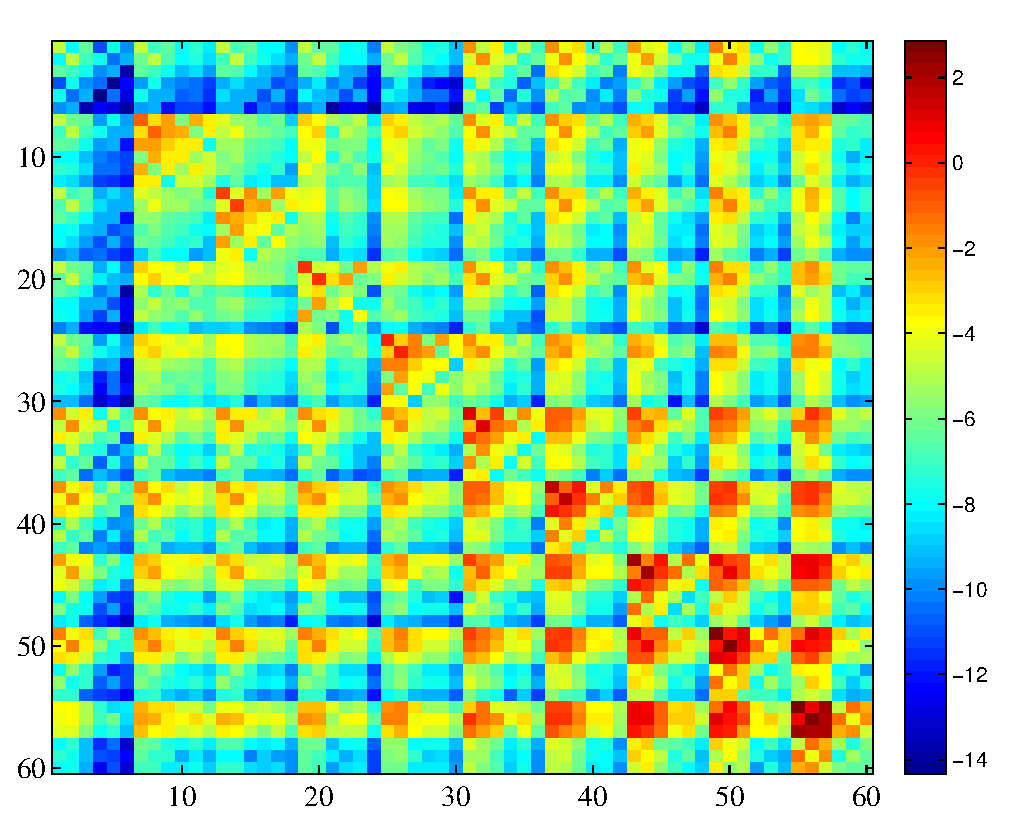
\includegraphics[width=5.5in]{./figures/covarianceEstimate}
 \caption[Solar system dynamic state covariance estimate]{Covariance estimate for $\mf x_d$ (excluding gravitational parameters) for the sun, solar system planets, and pluto, calculated as in \refeq{eq:covEst}.  The colorbar is in log scale (base 10), representing the absolute covariance magnitudes.  The block structure arises from cross-correlations between parameters associated with specific bodies, creating $6 \times 6$ blocks with $3 \times 3$ sub-blocks for position and velocity states. \label{fig:covarianceEstimate}}
\end{figure} 

Because so much of the original (pre-Kepler) exoplanet data set is composed of doppler spectroscopy surveys it is useful to briefly discuss how exoplanet signals are extracted from these measurements.  As detailed in \S\ref{sec:rv_inst_obs} doppler spectroscopy measures the  radial component of a star's velocity.  Planet signals may be identified by finding periodicities in this velocity (or analogously, in the star's position as found by precision astrometry).  This is usually accomplished via a periodogram (Fourier spectrum) analysis.  For an evenly sampled set of data points $\{x_j\}_{j=1}^N$, the discrete Fourier transform (DFT) is given by:
\begin{equation}
\hat{\mf x} = \mf F \mf x
\end{equation}
where $\mf x$ is the column vector of $x_i$ values and $\mf F$ is the Fourier matrix defined as:
\begin{equation}
\left[\mf F\right]_{mn} = \frac{1}{\sqrt{N}}e^{-2\pi i m n/N} \,.
\end{equation}
As long as the data is evenly sampled, the set $\{j/N\}_{j=1}^N$ represents the Fourier frequencies which will include all of the strong periodicities found in the data set and whose spectral power can be calculated as:
\begin{equation}
P_j = 2\left\vert \left[\hat{\mf x}\right]_j \right\vert^2 \,.
\end{equation}
Since the DFT produces a vector $\hat{\mf x}$ such that:
\begin{equation}
\left[\hat{\mf x}\right]_j = \left[\hat{\mf x}\right]_{N-j}^\star
\end{equation}
where $[\cdot]^\star$ represents the complex conjugate, the periodogram is only computed for the first half of the matrix.

Unfortunately, in most cases it is difficult to achieve an astronomical data set with completely even sampling due to all of the various target observability effects discussed in \S\ref{sec:targ_selection}.  One method  for dealing with this, very commonly found in the literature \citep{black1982, scargle1982, cumming2003, sozzetti2005, cumming2008} is the Lomb-Scargle periodogram.  For a set of data points $\{x_j\}_{j=1}^N$ collected at times $\{t_j\}_{j=1}^N$ with sample mean $\bar x$ and sample variance $\sigma^2$, the Lomb-Scargle periodogram defines the spectral power (as a function of angular frequency $\omega$) as:
\begin{equation}
\begin{split}
P_N(\omega) = \frac{1}{2\sigma^2} &\left[ \frac{\left(\sum_{j=1}^N \left( x_j - \bar x\right) \cos\left(\omega(t_j - \tau)\right)\right)^2}{\sum_{j=1}^N \cos^2\left(\omega(t_j - \tau)\right)}\right.\\
&\left.{} + \frac{\left(\sum_{j=1}^N \left( x_j - \bar x\right) \sin\left(\omega(t_j - \tau)\right)\right)^2}{\sum_{j=1}^N \sin^2\left(\omega(t_j - \tau)\right)}\right] \,,
\end{split}
\end{equation}
where the time offset $\tau$ for each $\omega$ is determined by:
\begin{equation}
\tau = \frac{1}{2\omega}\tan^{-1}\left(\frac{\sum_{j=1}^N \sin\left(2 \omega t_j\right)}{\sum_{j=1}^N \cos\left(2 \omega t_j\right)}\right) \,.
\end{equation}
The calculation of the time offset has two effects.  First, it makes the spectral power independent of any constant time shift.  Second, it makes the calculation of the periodogram equivalent to performing a least squares fit on the data to the simple harmonic model \citep{lomb1976least}:
\begin{equation}
x(t) = A \cos \omega t + B \sin \omega t \,,
\end{equation}
where the periodogram is the sum of the square of the coefficients:
\begin{equation}
P_N(\omega) = A^2 + B^2 \,.
\end{equation}

For any given angular frequency, the periodogram power, $P_N(\omega)$, has an exponential distribution function with unit mean for the case of the null hypothesis (i.e., that the data points represent independent Gaussian random values).  If we test $M$ independent frequencies then we can write the probability of finding a spectral power above some threshold value $P_0$ is given by:
\begin{equation}
P\left[P_N(\omega) > P_0\right] = 1 - \left(1 - e^{-P_0}\right)^M \,.
\end{equation}
This probability is equivalent to the false positive probability of the null hypothesis, and is therefore the significance level of $P_N(\omega)$.  The lower this value, the more significant the associated frequency.  This significance value scales approximately linearly with the number of independent frequencies $M$.  This value may be determined by Monte Carlo simulations where synthetic data sets of Gaussian deviates are generated for a fixed number of data points and the resulting periodogram values are fit for $M$.  Such experimentation has yielded the general result that $M$ is approximately equal to $N$ for approximately evenly sampled data, and when the range from zero to the Nyquist frequency is oversampled.  The value of $M$ differs from $N$ significantly only in cases where data points are closely clumped, in which case $M$ is reduced by a factor equal to the average clump size \citep{horne1986prescription,press1992numerical}.

Much effort has been devoted to finding fast implementations of the Lomb-Scargle periodogram, with one very popular method based on the fast Fourier transform (FFT) described in \citet{press1989fast}.  While these methods can be made accurate to any desired precision, modern computers are fully capable of calculating the exact periodogram for data sets of several thousand points.  A sample implementation of this algorithm is presented in \refcode{code:LombScargle}.  In cases where astrometric or radial velocity data is available, the periodogram can be very valuable in initializing the state by providing the number of planets in the system and their periods.  Furthermore, it is common practice to fit orbits directly to the significant periodogram frequencies, generating even better starting points for the filter \citep{sozzetti2002,sozzetti2003}.


\section{Updating the State}\label{sec:state_update}

\subsection{State Dynamics}
The system dynamics are governed by the orbital mechanics described in \S\ref{sec:exosystem_params}. Given the state defined in \refeq{eq:stateVector}, the system dynamics are governed by the ODE:
\begin{equation}\label{eq:state_update}
\dot{\mf x} = f(\mf x) = \begin{bmatrix}  {}^\mc I \mf v_{1/G} \\  -\sum\limits_{k \ne 1}\frac{\mu_k \R_{k/j}}{\Vert\R_{k/j}\Vert^3} \\ 0 \\ \vdots \\  {}^\mc I \mf v_{n/G} \\  -\sum\limits_{k \ne n}\frac{\mu_k \R_{k/j}}{\Vert\R_{k/j}\Vert^3} \\ 0 \\ \mathbf{0}_{c\times1}  \end{bmatrix}
\end{equation}
where $\mf r_{k/j} = \mf r_{k/G} - \mf r_{j/G}$, $c$ is the length of $\mf x_{c}$ and $n$ is the size of set $X$.

The Jacobian of $f(\mf x)$ can be decomposed into row blocks:
\begin{equation}
\mf F = \frac{\partial \mf f(\mf x)}{\partial \mf x} = \begin{bmatrix} \mf F_1 \\ \mf 0_{1\times 7n+c} \\ \mf F_2 \\ \mf 0_{1\times7n+c}\\ \vdots \\ \mf F_n \\ \mf 0_{c+1 \times 7n + c} \end{bmatrix}
\end{equation}
where:
\begin{equation}
\mf F_j = \begin{bmatrix}
\mathbf{0}_{3\times 3} & \mathbf{I} &  \mf 0_{3\times1} & \mathbf{0}_{3\times 3}  &  \mathbf{0}_{3\times 3} & \mf 0_{3\times1} & \cdots & \mathbf{0}_{3\times 3} & \mathbf{0}_{3\times 3} & \mathbf{0}_{3\times c} \\
\mf F_{j1} &  \mathbf{0}_{3\times 3} & \mf G_{j1} & \mf F_{j2} & \mathbf{0}_{3\times 3} & \mf G_{j2} &  \cdots & \mf F_{jn} & \mf G_{jn} &  \mathbf{0}_{3\times c} \end{bmatrix} \, .
\end{equation}

The submatrices $\mf F_{jk}$ are the partial derivatives of \ref{eq:nbody} with respect to the position vectors and the submatrices $\mf G_{jk}$ are the partial derivatives with respect to the gravitational parameters. Taking $\mf r_{k/G} =  \left[ \begin{array}{ccc} r_{k1} & r_{k2} & r_{k2} \end{array}\right]^T$ and $\mf r_{j/G} =  \left[ \begin{array}{ccc} r_{j1} & r_{j2} & r_{j2} \end{array}\right]^T$, we have:
\begin{equation}
\mf r_{k/j} =  \begin{bmatrix} r_{k1} - r_{j1} \\ r_{k2} - r_{j2} \\ r_{k3} - r_{j2} \end{bmatrix}= \begin{bmatrix} r_{kj_1} \\ r_{kj_2} \\ r_{kj_2} \end{bmatrix} \,.
\end{equation} 
This allows us to write:
\begin{equation}
\mf F_{jk} =
\begin{cases}
  - \sum\limits_{k \ne j} \mu_k \begin{bmatrix}
\dfrac{3r_{kj_1}^2}{\vert \R_{k/j} \vert^5} - \dfrac{1}{\vert \R_{k/j} \vert^3} & \dfrac{3r_{kj_1}r_{kj_2}}{\vert \R_{k/j} \vert^5} & \dfrac{3r_{kj_1}r_{kj_3}}{\vert \R_{k/j} \vert^5}\\
\dfrac{3r_{kj_1}r_{kj_2}}{\vert \R_{k/j} \vert^5}  &  \dfrac{3r_{kj_2}^2}{\vert \R_{k/j} \vert^5} - \dfrac{1}{\vert \R_{k/j} \vert^3}  & \dfrac{3r_{kj_2}r_{kj_3}}{\vert \R_{k/j} \vert^5}\\
\dfrac{3r_{kj_1}r_{kj_3}}{\vert \R_{k/j} \vert^5} &  \dfrac{3r_{kj_2}r_{kj_3}}{\vert \R_{k/j} \vert^5} & \dfrac{3r_{kj_3}^2}{\vert \R_{k/j} \vert^5} - \dfrac{1}{\vert \R_{k/j} \vert^3}  \end{bmatrix} &
j \ne k \\\\
\hspace{5.5ex} \mu_k \begin{bmatrix}
\dfrac{3r_{kj_1}^2}{\vert \R_{k/j} \vert^5} - \dfrac{1}{\vert \R_{k/j} \vert^3} & \dfrac{3r_{kj_1}r_{kj_2}}{\vert \R_{k/j} \vert^5} & \dfrac{3r_{kj_1}r_{kj_3}}{\vert \R_{k/j} \vert^5}\\
\dfrac{3r_{kj_1}r_{kj_2}}{\vert \R_{k/j} \vert^5}  &  \dfrac{3r_{kj_2}^2}{\vert \R_{k/j} \vert^5} - \dfrac{1}{\vert \R_{k/j} \vert^3}  & \dfrac{3r_{kj_2}r_{kj_3}}{\vert \R_{k/j} \vert^5}\\
\dfrac{3r_{kj_1}r_{kj_3}}{\vert \R_{k/j} \vert^5} &  \dfrac{3r_{kj_2}r_{kj_3}}{\vert \R_{k/j} \vert^5} & \dfrac{3r_{kj_3}^2}{\vert \R_{k/j} \vert^5} - \dfrac{1}{\vert \R_{k/j} \vert^3}  \end{bmatrix} & j = k
\end{cases}
\end{equation}
and
\begin{equation}
\mf G_{jk} =
\begin{cases}
 -\frac{\R_{k/j}}{\Vert\R_{k/j}\Vert^3} &
j \ne k \\
\mf 0_{3\times 1} & j = k \,.
\end{cases}
\end{equation}

Since numerical integration of \refeq{eq:stateCovIntegration} requires a first order integrator, the Runge-Kutta-Nystr\"{o}m integrators cannot be used to propagate the state and covariance and must be replaced with a first order symplectic integrator.  Because of the large quantities of zero entries in the Jacobians, a sparse matrix encoding is often used to increase filtering efficiency.

\subsection{Observation Equations}
In order to write the observation functions for the various detection methods discussed in \refch{ch:obs_methods}, we must first decide what to count as the observation for each method.  We could start with the absolute raw form of each measurement, such as pixel data numbers for imaging, or uncalibrated photon counts for transit photometry, but this would place a significant extra burden on the filter by making all of the observation equations highly nonlinear and requiring an additional set of parameters (beyond the ones already defined) to map the observations to the state.  More importantly, each detection method has a well-developed set of tools for processing the raw data.  These have been developed and tested over many years, and so we can have a high degree of confidence in their outputs. Therefore, we will assume that the standard processing typically applied to each observation has been performed and use that as a starting point.  This could potentially introduce additional noise sources into the data sets, but as long as these can be characterized and incorporated into the appropriate $\mf R$ covariances this should not have a large effect on the filter performance.  Thus we take the observations to be:
\begin{align}
\mf z_{dd} &= \begin{bmatrix} \mf s \\ \frac{F_P}{F_S} \end{bmatrix} \,,\\
\mf z_{ast} &= \begin{bmatrix} \mf b_1 \cdot \left(\hat{\mf r}_{S/sc} - \hat{\mf r}_{c/sc}\right) \\\mf b_2 \cdot \left(\hat{\mf r}_{S/sc} - \hat{\mf r}_{c/sc}\right) \end{bmatrix} B \,,\\
\mf z_{rv} &=  \mf r_{S/G}\,,\\
\mf z_{phot} &= \frac{F_P}{F_S}\,,
\end{align}
for direct detection, astrometry,\footnote{Since the baseline length, $B$, and orientations $\mf b_i$ are properties of the instrument, we assume that these are known parameters and do not include them into the state.  However, since the orientation knowledge for a real astrometric space-based observatory would be built up over the course of many observations \citep{murphy2004} an alternate filter formulation designed to run before the mission had completed would need to include the orientation vectors in the state.} doppler spectroscopy, and transit photometry, respectively, with the appropriate noise terms added. Of these four, only doppler spectroscopy is fully linear in the state vector, whereas astrometry is the most highly nonlinear.  The corresponding Jacobian for direct detection is:
\begin{equation}
\mf H_{dd} = \begin{bmatrix}
\mf I_{2 \times 2} & \mf 0_{2 \times 7}\\
\mf H_z
\end{bmatrix}
\end{equation}
where
\begin{equation}
\mf H_z = 
\frac{p_jR_j^2 r_{j1}}{\pi r^4}\begin{bmatrix}
-\left(\sqrt{ r_{j1}^2 +  r_{j2}^2} + \pi  r_{j3} + 2  r_{j3}\sin^{-1}\left(r_{j3}/r\right) \right)\\
-\left(\sqrt{ r_{j1}^2 +  r_{j2}^2} + \pi  r_{j3} + 2  r_{j3}\sin^{-1}\left(r_{j3}/r\right) \right) \\
\left(-\sqrt{ r_{j1}^2 +  r_{j2}^2} r_{j3} + \left( r_{j1}^2 +  r_{j2}^2 -  r_{j3}^2\right)\left(\pi - \cos^{-1}\left(r_{j3}/r\right) \right)\right) \\
\mf 0_{4 \times 1} \\
\left(r^2/p_j\right)\left(\sqrt{ r_{j1}^2 +  r_{j2}^2}  + \pi r_{j3} - r_{j3}  \cos^{-1}\left(r_{j3}/r\right)\right) \\
\left(2r^2/R_j\right)\left(\sqrt{ r_{j1}^2 +  r_{j2}^2}  + \pi r_{j3} + r_{j3}  \sin^{-1}\left(r_{j3}/r\right)\right)
\end{bmatrix}
\end{equation}
for the compact state $\mf x = \begin{bmatrix} \mf r_{j/G}&  {}^\mc I \mf v_{j/G}& \mu_j& p_j& R_j \end{bmatrix}$ with $r = \Vert \mf r_{j/G} \Vert$.

Because the astrometric observation is so highly nonlinear, it is useful to try to find a to find a linearization (or low order series solutions) consistent with the original observation equation to the required level of precision.  The next section demonstrates the technique for doing so, using Earth-like planets to determine required precision.

\subsection{Astrometric Observation Function Linearization}\label{sec:expansion}
The classical approach to linearizing \refeq{eq:rhat_ssc} has been to expand about $\varpi$.  As we will see below, for the purposes of finding Earth-mass planets, these must necessarily include nonlinear terms, but an expansion is still useful as a simplifying step in the data analysis.  In order to decide which terms should be retained, we must first quantify the desired precision of the measurement.  There are several ways to do this, but a relatively straightforward one is to calculate the magnitude of the smallest signal we wish to be able to measure.  Following \citet{savransky2010simulation}, we will take as our smallest signal the effect of a single Earth-mass planet residing on an Earth-like orbit on the astrometric signature of a sun-twin star. 

\begin{figure}[ht]
\centering
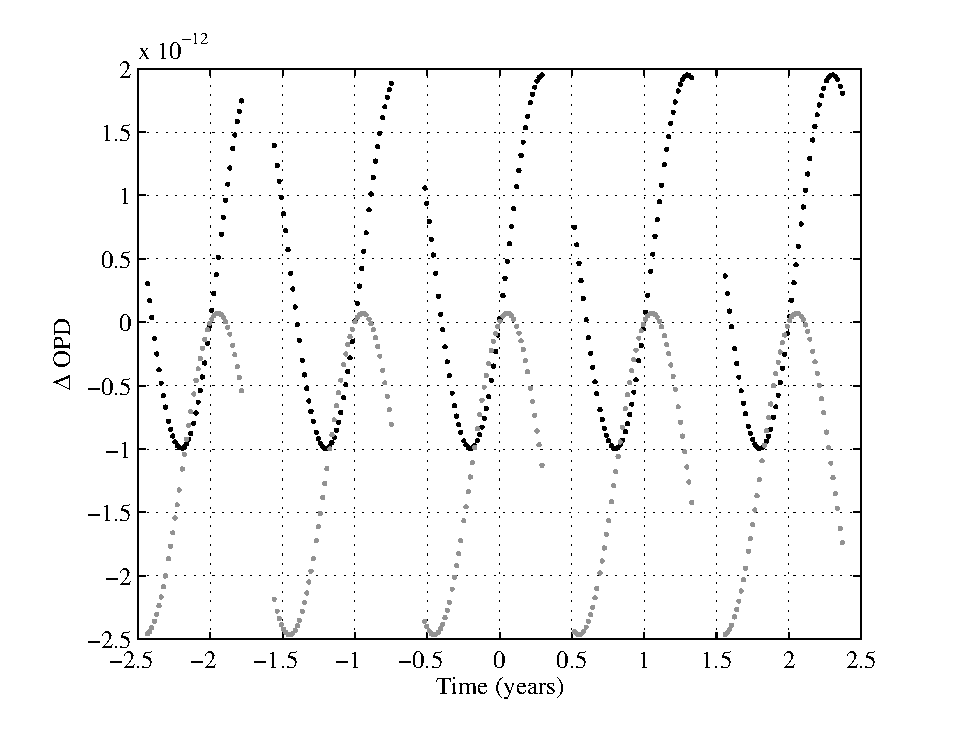
\includegraphics[width=5.5in]{./figures/planet_effects}
 \caption[Astrometric wobble due to Earth mass planet]{ Difference between differential OPDs (between a sun-twin star and fixed centroid) using exact expressions for $\hat\R_{s/sc}$ with and without the effects of an Earth-mass planet on an Earth-like orbit. The two curves represent the measurements along two orthogonal interferometer baseline orientations.\label{fig:planet_effects}}
\end{figure} 
\reffig{fig:planet_effects} shows the difference between the results of two simulations, each using \refeq{eq:rhat_ssc} and a fixed centroid position (with respect to the solar system barycenter).  The simulations include identical values for parallax, barycenter motion, and assume a sun-twin target star lying exactly 10 parsecs from the solar system barycenter (at epoch $t_0$). One simulation includes the stellar jitter due to an Earth-mass planet while the other does not\setcounter{footnote}{1}\footnote{The line of nodes of the planet's orbit is rotated by 45$^\circ$ with respect to the line of sight, producing the asymmetric magnitudes about 0 in the difference between differential OPDs}.  The difference between the two measurements is the most basic representation of the magnitude of the signal in which we are interested, and, in this case, shows a signal on the order of 1$\times10^{-12}$. This value is in the units of \refeq{eq:measurement}: it is the difference between fractions of the baseline distance. 

This tells us that to be sensitive to the jitter due to an Earth-twin with any measure of confidence, we must retain all terms in the measurement of order 1$\times10^{-13}$ or greater (assuming that our analysis technique will be sensitive to structured signals up to one order of magnitude below the target signal).  To aid in this calculation, \reftable{tbl:typ_vals} enumerates the ranges of typical values for the various terms in \refeq{eq:rhat_ssc}.
\begin{table}[ht]
\caption[Typical values of terms in astrometric observation equation]{Typical values for terms in \refeq{eq:rhat_ssc}.\label{tbl:typ_vals}}
\begin{center}
\begin{threeparttable}[b]
\begin{tabular}{ c c l}
\hline\hline
Term & Typical Order & Notes \\
\hline
$a_0$ & 1 & All distances are assumed to be in AU\\
$\hat\R_s(t_0)$ & 1 &\\
$\bar\R_\mu$\tnote{*} & 5$\times10^{-6}$/year & Barnard's star is 5$\times10^{-5}$/year \\
$\Delta \tilde\R_{s/G}$ & 1$\times10^{-6}$ to 1$\times10^{-2}$ & For solar system planets \\
\multirow{2}{*}{$ \tilde\R_{sc}$} & \multirow{2}{*}{1} & Assuming a ground-based, Earth orbiting\\
& & or Earth-trailing spacecraft\\
$\varpi $& 5$\times10^{-6}$ to 5$\times10^{-8}$ & For target distance of 1-100 parsecs.\\
\hline
\end{tabular}
\begin{tablenotes}
\item[*]While $\bar\R_\mu$ is a time dependent value, for measurements made over a span of 5 to 10 years it will change by less than one order, so we will assume a conservative, constant value when considering which terms to keep in our expansions.
\end{tablenotes}
\end{threeparttable}
\end{center}
\end{table}

We begin the expansion by dividing the numerator and denominator of \refeq{eq:rhat_ssc} by $\|\R_s(t_0)\|$ to write the normalized version of the equation:
%
\begin{equation} \label{eq:rhat_norm}
\begin{split}
\hat\R_{s/sc} &= (\hat\R_s(t_0) + \bar\R_\mu +\varpi\Delta \tilde\R_{s/G}- \varpi\tilde\R_{sc})\times\\ 
&\hspace{2.5ex}\left\{ 1 + \bar\R_\mu \cdot \bar\R_\mu + \varpi^2\Delta \tilde\R_{s/G} \cdot \Delta \tilde\R_{s/G} +\varpi^2\tilde\R_{sc} \cdot \tilde\R_{sc}  + 2\hat\R_s(t_0) \cdot \bar\R_\mu \right.\\
&\hspace{3ex}{ }+ 2 \varpi \hat\R_s(t_0) \cdot \Delta \tilde\R_{s/G} - 2\varpi\hat\R_s(t_0) \cdot \tilde\R_{sc}  + 2\varpi \bar\R_\mu \cdot  \Delta \tilde\R_{s/G}\\
&\hspace{3ex}{} - 2\varpi \bar\R_\mu \cdot \tilde\R_{sc} - 2\varpi^2 \Delta \tilde\R_{s/G} \cdot \tilde\R_{sc} \left. \right\}^{-\frac{1}{2}}
\end{split}
\end{equation}
where $\bar\R_\mu = \R_\mu/\|\R_s(t_0)\|$, $\tilde\R_{sc}$ is the spacecraft position normalized by $a_0$ and $\Delta \tilde\R_{s/G}$ is  $\Delta \R_{s/G}$ normalized by $a_0$.  

We next apply a binomial expansion to the denominator of \refeq{eq:rhat_norm} and retain terms explicitly in $\varpi$ to first order.  Since the signal we are looking for appears explicitly only as $\varpi\Delta \tilde\R_{s/G}$, any terms of proportional order must be retained.  Thus, terms proportional to $\Vert \bar\R_\mu \Vert^2$ must be left in, but terms proportional to $\Vert \bar\R_\mu \Vert^n$ for $n > 2$ and terms proportional to $\Vert \bar\R_\mu \Vert^n\varpi$ for $n > 1$ are dropped.  We also drop all terms proportional to $\hat\R_s(t_0)$, as dotting $\hat\R_{s/sc}$ with $\mf b_i$ as in the measurement \refeq{eq:measurement} causes these terms to equal zero.  The resulting approximation is:
\begin{equation}\label{eq:rhat_expand1}
\begin{split}
\hat\R_{s/sc}\cdot &\mf b_i \approx
\left\{\bar\R_\mu  - (\hat\R_s(t_0) \cdot \bar\R_\mu)\bar\R_\mu +  \left[\Delta \tilde\R_{s/G}  - \tilde \R_{sc}  -(\hat\R_s(t_0)\cdot\bar\R_\mu)\Delta \tilde\R_{s/G}\right.\right.\\
&\left.\left.{} + (\hat\R_s(t_0) \cdot \tilde\R_{sc}) \bar\R_\mu - (\Delta\tilde\R_{s/G} \cdot \hat\R_s(t_0))\bar\R_\mu +(\hat\R_s(t_0)\cdot\bar\R_\mu)\tilde \R_{sc}\right]\varpi \right\} \cdot \mf b_i \,.
\end{split}
\end{equation}
This is  a linear expression in parallax and can be used to extract the stellar reflex signal, though it contains complicated couplings among the spacecraft position, parallax, barycenter motion, and stellar reflex.  Note that it is not assumed that these other terms are known; rather, the barycenter motion and the parallax factor, $\varpi$, must also be estimated in the data analysis.  This leads to the problem of attempting to fit the radial motion of the target from purely astrometric measurements.  While the radial and proper motions of targets are approximated as completely separate in the classical treatment, the level of precision required for this application means that we must consider the effects of radial motion.  The first term of \refeq{eq:rhat_expand1} is $\bar\R_\mu \cdot \mf b_i$.  If $\mf b_i$ is, as was assumed in \S\ref{sec:ast_inst_obs}, equivalent to $\mf b_1$ or $\mf b_2$, then the $\sigma_z$ dependence of this term is exactly zero.  Similarly, the next two terms in the direction of $\bar\R_\mu$ will have no $\sigma_z$ components when dotted with $\mf b_i$.  However, the two final terms in this expansion have magnitudes given by $\varpi  (\hat\R_s(t_0)\cdot\bar\R_\mu)$, which makes them proportional to $\sigma_z$.  As these two terms are in the directions of $ \tilde \R_{sc}$ and $\Delta \tilde\R_{s/G}$, which are arbitrarily oriented in the tangent frame, this $\sigma_z$ dependence is not zeroed even when the baseline is perfectly aligned with $\mf b_1$ or $\mf b_2$.  Thus, the radial star motion explicitly enters our expression, and makes a significant contribution at the desired level of precision.

\begin{figure}[ht]
\centering
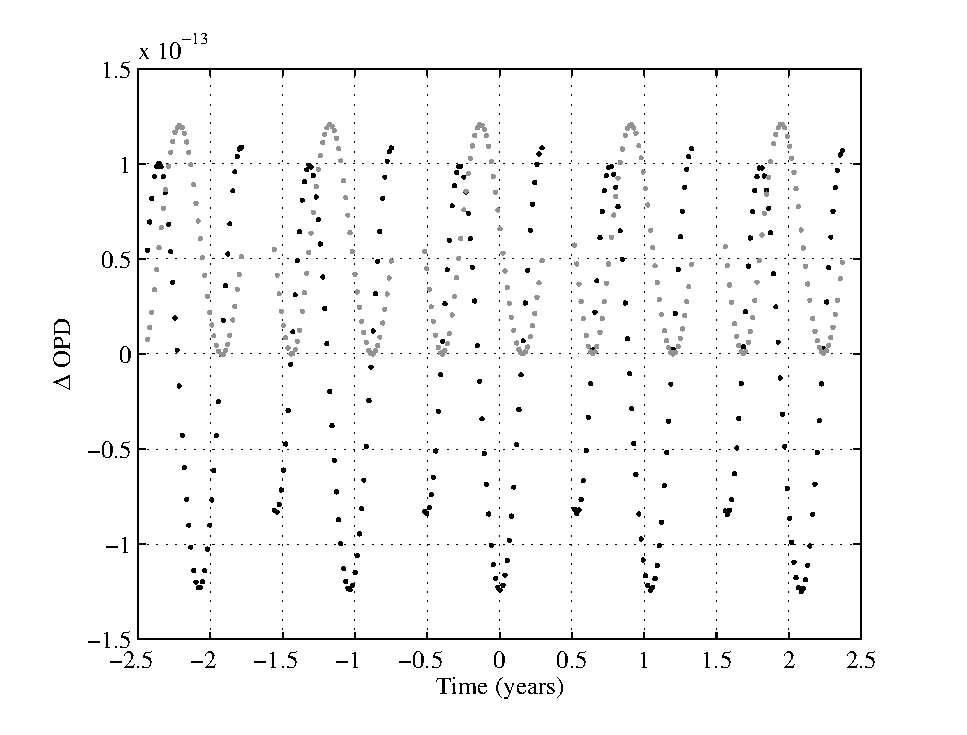
\includegraphics[width=5.5in]{./figures/first_order_expansion}
 \caption[First order expansion of astrometric observation]{ Difference between differential OPDs (between a sun-twin star and fixed centroid) using the exact expression for $\hat\R_{s/sc}$ and the first order expansion from \refeq{eq:rhat_expand1}. The two curves represent the measurements along two orthogonal interferometer baseline orientations.\label{fig:first_order_expansion}}
 \end{figure}
\reffig{fig:first_order_expansion} repeats the simulation from \reffig{fig:planet_effects}, including the planet in both cases, but now comparing the exact expression for $\hat\R_{s/sc}$ and the first order expansion in \refeq{eq:rhat_expand1}.  The resulting error is less than one order of magnitude below the signal due to the planet, which means that it is of the same order as the desired sensitivity for all targets closer than 10 pc or with any combination of the other parameters which would cause the planet signal to decrease in magnitude.  Additionally, the structure of the error is dominated by parallax terms, which produce periodic structure that could be mistaken for astrometric wobble due to another planet.  We can compare \refeq{eq:rhat_expand1} with previously published first-order forms such as Equations 31 and 32 in \citet{konacki2002frequency}.  These are quite similar in form to the expression derived here, except that Konacki assumes that all radial components of motion are unobservable, and thus the equivalent vectors to $\Delta \tilde\R_{s/G}$ and $\bar\R_\mu$ are formed without the $\hat\R_s(t_0)$ components.  Konacki's expression also does not subtract the initial displacement of the target star from its system's barycenter, thereby applying the proper motion to the star rather than the system barycenter.  If we redo our simulation using the first order expansion with the radial terms dropped, we end up with residuals one order of magnitude higher than those in \reffig{fig:first_order_expansion}.  Thus, the exclusion of radial terms produces residuals that are one order of magnitude above the target signal, rather than one order of magnitude below, as seen in \reffig{fig:first_order_expansion_norv}.
\begin{figure}[ht]
\centering
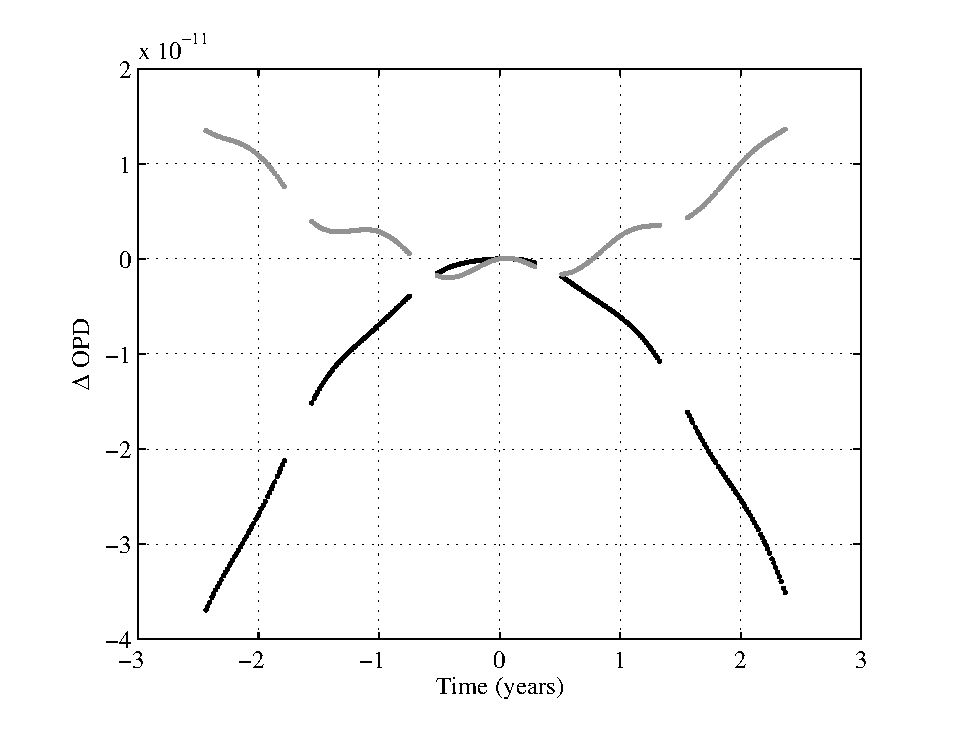
\includegraphics[width=5.5in]{./figures/first_order_expansion_norv}
 \caption[First order expansion of astrometric observation without radial velocity terms]{Difference between differential OPDs (between a sun-twin star and fixed centroid) using the exact expression for $\hat\R_{s/sc}$ and the first order expansion from \refeq{eq:rhat_expand1} with the radial terms neglected. The two curves represent the measurements along two orthogonal interferometer baseline orientations.\label{fig:first_order_expansion_norv}}
 \end{figure}
 
Furthermore, a number of the terms dropped in this expansion were proportional to $\varpi^2$ multiplied by quantities of order 1.  The astrometric literature is quite clear that a first order expansion in $\varpi$ is only good to milliarcsec accuracy \citep{green1985spherical}.  If an astrometric instrument has a final precision of sub-$\mu$arcsec, it is important to ask if measurable terms were dropped in the expansion.  Such terms can get as large as 6 times $\varpi^2$.  Again, for a star at 10 pc, $\varpi \sim 5 \times 10^{-7}$, making the second order terms of order $2.5 \times 10^{-13}$.   Thus, for most stars the approximation is a good one but it does raise concerns for the closest targets, or for analysis methods that are sensitive to non-random signals just below the level of the target signal.  

To address this, we can repeat the expansion to second order in $\varpi$.  However, for consistency, we must now retain some additional terms.  The zeroth and first order terms (in $\varpi$) remain the same (since $\Vert \bar\R_\mu \Vert^3$ is of order 1$\times10^{-16}$ and  $\Vert \bar\R_\mu \Vert^2\varpi$ is of order 1$\times10^{-17}$).  Any terms in $\varpi^2$ with factors of $\bar\R_\mu$ can safely be dropped.  Terms in $\varpi^2$ with factors of $\Delta \tilde\R_{s/G}$ should also be quite small, but we will leave these to first order since it is theoretically possible that there exist systems with both Earth-like planets and very large, widely separated super-Jupiters which have not yet been detected by RV (due to their very long periods), and which would cause a large stellar reflex to make these factors significant.  These considerations leave only three new terms in the expansion:
\begin{equation}\label{eq:rhat_expand2}
\begin{split}
\hat\R_{s/sc}\cdot &\mf b_i \approx
\left\{\bar\R_\mu  - (\hat\R_s(t_0) \cdot \bar\R_\mu)\bar\R_\mu +  \left[\Delta \tilde\R_{s/G}  - \tilde \R_{sc}  -(\hat\R_s(t_0)\cdot\bar\R_\mu)\Delta \tilde\R_{s/G}\right.\right.\\
&{} + \left.(\hat\R_s(t_0) \cdot \tilde\R_{sc}) \bar\R_\mu - (\Delta\tilde\R_{s/G} \cdot \hat\R_s(t_0))\bar\R_\mu +(\hat\R_s(t_0)\cdot\bar\R_\mu)\tilde \R_{sc}\right]\varpi\\
&{} + \left[\tilde\R_{sc} (\hat\R_s(t_0) \cdot \Delta \tilde\R_{s/G}) + \Delta \tilde\R_{s/G} (\hat\R_s(t_0) \cdot \tilde\R_{sc}) \right.\\
&\left.\left.{} - \tilde\R_{sc} (\hat\R_s(t_0) \cdot \tilde\R_{sc})\right]\varpi^2\right\} \cdot \mf b_i \,.
\end{split}
\end{equation}

 \begin{figure}[ht]
\centering
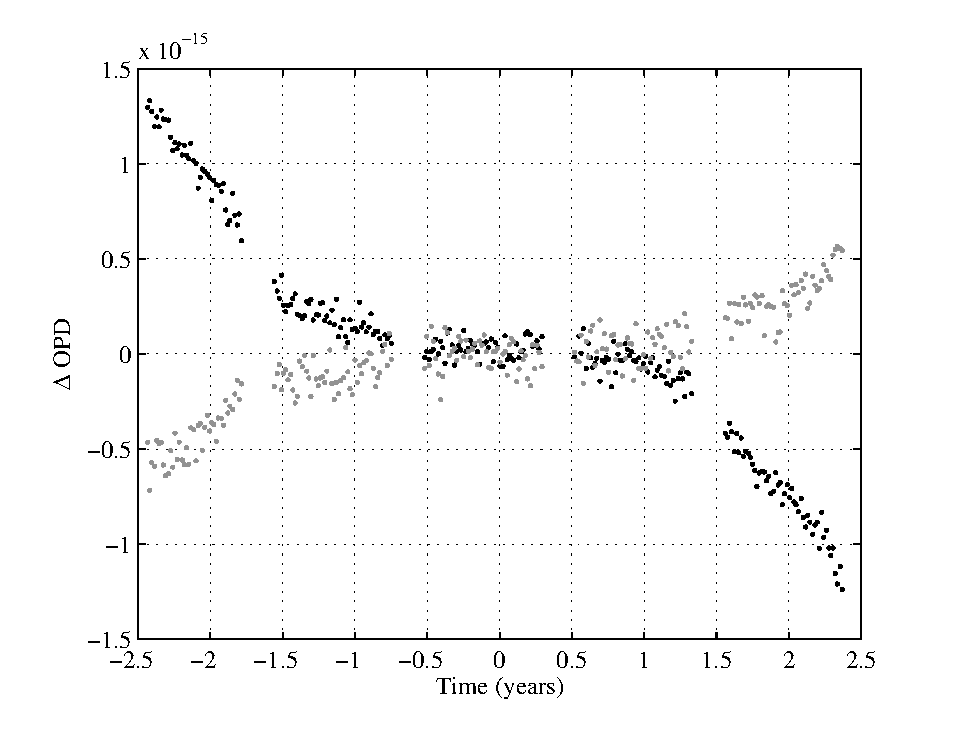
\includegraphics[width=5.5in]{./figures/second_order_expansion}
 \caption[Second order expansion of astrometric observation equation]{ Difference between differential OPDs (between a sun-twin star and fixed centroid) using the exact expression for $\hat\R_{s/sc}$ and the second order expansion from \refeq{eq:rhat_expand2}. The two curves represent the measurements along two orthogonal interferometer baseline orientations. \label{fig:second_order_expansion}}
\end{figure} 
\reffig{fig:second_order_expansion} shows the difference between the exact expression for $\hat\R_{s/sc}$ and the second order expansion in  \refeq{eq:rhat_expand2}.  The resulting error is now two to three orders of magnitude below the target signal.  The error structure is now dominated by proper motion terms, which are linear, not periodic.  These could still be confused with the effects of long period planets, but the signals are so low compared to the target signal that this possibility is unlikely.  It is important to note, however, the fitting problem has become significantly more challenging as the parameters enter nonlinearly in the measurement.

The practice of dropping terms that are in the direction of $\hat\R_s(t_0)$ breaks down in two cases: when there is pointing error such that the interferometer baseline is not aligned with $\mf b_1$ or $\mf b_2$, or when expressing the direction to a different star (i.e., a non-ideal reference source) in the tangent frame defined by the target star.  In these cases, a number of additional terms must be included in our expansion.  Following the same procedure as above, we can rewrite \refeq{eq:rhat_expand2} as:
\begin{equation}\label{eq:rhat_expand2_perr}
\begin{split}
\hat\R_{s/sc} \approx&
\hat\R_s(t_0) + \bar\R_\mu - \hat\R_s(t_0) (\hat\R_s(t_0) \cdot \bar\R_\mu) - \bar\R_\mu (\hat\R_s(t_0) \cdot \bar\R_\mu) -  \frac{1}{2} \hat\R_s(t_0)(\bar\R_\mu \cdot \bar\R_\mu)\\
&{} + \frac{3}{2} \hat\R_s(t_0)(\hat\R_s(t_0) \cdot \bar\R_\mu)^2  + \left[\vphantom{\frac{1}{2}}\Delta \tilde\R_{s/G} - \tilde\R_{sc} - \Delta \tilde\R_{s/G} (\hat\R_s(t_0) \cdot \bar\R_\mu) + \tilde\R_{sc} (\hat\R_s(t_0) \cdot \bar\R_\mu) \right.\\
&{}  - \hat\R_s(t_0) (\hat\R_s(t_0) \cdot \Delta \tilde\R_{s/G}) - \bar\R_\mu (\hat\R_s(t_0) \cdot \Delta \tilde\R_{s/G}) + \hat\R_s(t_0) (\hat\R_s(t_0) \cdot \tilde\R_{sc})\\
&{} + 3\hat\R_s(t_0) (\hat\R_s(t_0) \cdot \bar\R_\mu) (\hat\R_s(t_0) \cdot \Delta \tilde\R_{s/G}) + \bar\R_\mu (\hat\R_s(t_0) \cdot \tilde\R_{sc}) \\
&\left.{}  - 3\hat\R_s(t_0) (\hat\R_s(t_0) \cdot \bar\R_\mu) (\hat\R_s(t_0) \cdot \tilde\R_{sc}) - \hat\R_s(t_0) (\bar\R_\mu \cdot \Delta \tilde\R_{s/G}) + \hat\R_s(t_0) (\bar\R_\mu \cdot \tilde\R_{sc})\vphantom{\frac{1}{2}}\right] \varpi  \\
&{}+ \left[\vphantom{\frac{1}{2}}\tilde\R_{sc} (\hat\R_s(t_0) \cdot \Delta \tilde\R_{s/G}) + \Delta \tilde\R_{s/G} (\hat\R_s(t_0) \cdot \tilde\R_{sc}) - \tilde\R_{sc} (\hat\R_s(t_0) \cdot \tilde\R_{sc})\right.\\
&{} - 3\hat\R_s(t_0) (\hat\R_s(t_0) \cdot \Delta \tilde\R_{s/G}) (\hat\R_s(t_0) \cdot \tilde\R_{sc}) + \hat\R_s(t_0) (\Delta \tilde\R_{s/G} \cdot \tilde\R_{sc})\\
&\left.{} - \frac{1}{2} \hat\R_s(t_0)(\tilde\R_{sc} \cdot \tilde\R_{sc})  + \frac{3}{2} \hat\R_s(t_0)(\hat\R_s(t_0) \cdot \tilde\R_{sc})^2\right] \varpi^2
\end{split}
\end{equation}
where the subscript $s$ may now refer to either the target star, or any of its reference sources.

We now have a completely general second order expansion of the spacecraft to source unit vector, which applies when the source is different from the target star used to define the tangent frame, or when the spacecraft baseline pointing does not coincide with the vectors of the tangent frame.  In the first case, we retain terms proportional to $\hat\R_s(t_0) \cdot \mf b_i$ because $\hat\R_s(t_0) \ne \mf b_3$ and so these terms do not automatically go to zero.  In the second case, these terms do not go to zero because $\mf b_i \ne \mf b_1$ or $\mf b_2$.  This expression is even more complex than \refeq{eq:rhat_expand2}, and even less suitable for use in analysis.  However, this added complexity is actually mitigated by the same reasons that caused us to add in the extra terms.  First, if the pointing error is small (i.e., the baseline is reasonably close to one of the two tangent frame unit vectors), then only the new terms in $\hat\R_s(t_0)$ whose coefficients are of order 1 should be kept, as $\hat\R_s(t_0) \cdot \mf b_i$ will still represent a small value.  Second, even non-ideal reference sources will still usually be stars which are significantly further from the solar system than the target star, with much smaller parallax and barycenter motion values.  As such, the first order form will typically be sufficiently precise for these sources, allowing most or all of the terms in $\varpi^2$ to be dropped.

Another way to simplify these equations is to note that we have so far been assuming no prior knowledge of the astrometric quantities ($\varpi, \bar\R_\mu$) being measured.  In reality we already have some knowledge of the barycenter motion and parallax of our target stars, and high precision astrometric observations will be used to update, rather than replace existing measurements.  To represent this, we can rewrite \refeq{eq:rhat_norm}
with $\bar\R_{\mu}$ replaced by $\bar\R_{\mu0}+ \delta\bar\R_\mu$ and $\varpi$ replaced by $\varpi_0 + \delta\varpi$, where $\bar\R_{\mu0}$ and $\varpi_0$ are the currently known components of barycenter motion and parallax and $\delta\bar\R_\mu$ and $\delta\varpi$ are the (relatively small) correction terms. The result is:
\begin{equation}\label{eq:rhat_norm2}
\begin{split}
\hat\R_{s/sc} &= (\hat\R_s(t_0) + \bar\R_{\mu0} + \delta\bar\R_\mu  +(\varpi_0 + \delta\varpi)\Delta \tilde\R_{s/G} - (\varpi_0 + \delta\varpi)\tilde\R_{sc})\times  \\
&\left\{1 + \bar\R_{\mu0} \cdot \bar\R_{\mu0} + \delta\bar\R_\mu \cdot \delta\bar\R_\mu + 2 \bar\R_{\mu0} \cdot \delta\bar\R_\mu + (\varpi_0 + \delta\varpi)^2\Delta \tilde\R_{s/G} \cdot \Delta \tilde\R_{s/G}\right.\\
 &{} + (\varpi_0 + \delta\varpi)^2\tilde\R_{sc} \cdot \tilde\R_{sc} + 2\hat\R_s(t_0) \cdot \bar\R_{\mu0} + 2\hat\R_s(t_0) \cdot \delta\bar\R_\mu \\
 &{} + 2 (\varpi_0 + \delta\varpi) \hat\R_s(t_0) \cdot \Delta \tilde\R_{s/G} - 2(\varpi_0 + \delta\varpi)\hat\R_s(t_0) \cdot \tilde\R_{sc} \\
 &{}  +  2(\varpi_0 + \delta\varpi) (\bar\R_{\mu0}  \cdot  \Delta \tilde\R_{s/G} + \delta\bar\R_\mu \cdot  \Delta \tilde\R_{s/G} )\\
&\left.{} - 2(\varpi_0 + \delta\varpi) (\bar\R_{\mu0}\cdot \tilde\R_{sc} + \delta\bar\R_\mu\cdot \tilde\R_{sc}) - 2(\varpi_0 + \delta\varpi)^2 \Delta \tilde\R_{s/G} \cdot \tilde\R_{sc}\right\}^{-\frac{1}{2}}
\end{split}
\end{equation}

In order to carry out expansions as before, it is necessary to quantify the expected values of these new variables so that we can decide which terms are negligible and which are important.  Since we are assuming that our a priori estimates will be reasonably good, $\bar\R_{\mu0}$ and $\varpi_0$ should be of the same order as $\R_\mu$ and $\varpi$ above.  Currently, parallax and proper motion are known to at least 1 mas and 1 mas/year accuracy, respectively \citep{turon1995}.  We will take  $\delta\varpi$ to be of order 5$\times10^{-9}$; $\Vert\delta\bar\R_\mu\Vert$ will vary in magnitude in time, but could be of order 1$\times10^{-8}$ within five years of observations.  

We again perform a binomial expansion on the denominator of equation (\ref{eq:rhat_norm2}) and retain terms explicitly in $\varpi_0$ to second order and explicitly in $\delta\varpi$ to first order.   As before, terms proportional to $\Vert \bar\R_{\mu0} \Vert^n$ for $n > 2$ and terms proportional to $\Vert \bar\R_{\mu0} \Vert^n\varpi_0$ for $n > 1$ are dropped, as are terms proportional to  $\Vert \delta\bar\R_{\mu} \Vert^n$ for $n > 1$, terms proportional to $\Vert \delta\bar\R_{\mu} \Vert\delta\varpi$, and terms including $\varpi^2$ that are proportional to $\Vert\Delta \tilde\R_{s/G}\Vert^n$ for $n>1$.

Terms proportional to $\Vert \bar\R_{\mu0} \Vert \delta\varpi$, $\Vert \bar\R_{\mu0} \Vert\Vert \delta\bar\R_{\mu} \Vert$, and $\Vert \delta\bar\R_{\mu} \Vert\varpi_0$ are borderline---for the values assumed here, they have magnitudes of up to 1$\times10^{-14}$, which means they should be neglected, but if the proper motions are larger than expected (or there is higher uncertainty in the a priori measurements), then these terms can become significant, so we will leave them.  Similarly, terms proportional to $\varpi_0\delta\varpi$  have magnitudes of 1$\times10^{-15}$ for the values assumed here, and are fairly unlikely to become significant unless uncertainties in parallax are much greater than expected for the nearest stars.  We include only one of these terms because leaving it out leaves a clear sinusoidal pattern in the signal of order 5$\times10^{-15}$.  If the chosen analysis method is not expected to be sensitive to  such a signal, this term can safely be omitted.  The resulting approximation is:
\begin{equation} \label{eq:rhat_expand_apri}
\begin{split}
\hat\R_{s/sc} \cdot \mf b_i &\approx
\left\{\bar\R_{\mu0} + \delta\bar\R_\mu - \bar\R_{\mu0} (\hat\R_s(t_0) \cdot \bar\R_{\mu0}) - \delta\bar\R_\mu (\hat\R_s(t_0) \cdot \bar\R_{\mu0}) \right.\\
&{}- \bar\R_{\mu0} (\hat\R_s(t_0) \cdot \delta\bar\R_\mu) + \left[\vphantom{1}{2}\Delta \tilde\R_{s/G} - \tilde\R_{sc} - \Delta \tilde\R_{s/G} (\hat\R_s(t_0) \cdot \bar\R_{\mu0})\right. \\
&\left.{}+ \tilde\R_{sc} (\hat\R_s(t_0) \cdot \bar\R_{\mu0}) + \bar\R_{\mu0} (\hat\R_s(t_0) \cdot \tilde\R_{sc})\vphantom{1}{2}\right] \left(\delta\varpi +\varpi_0\right)\\
&{} - \bar\R_{\mu0} (\hat\R_s(t_0) \cdot \Delta \tilde\R_{s/G})\delta\varpi + \left[ \tilde\R_{sc} (\hat\R_s(t_0) \cdot \delta\bar\R_\mu) + \delta\bar\R_\mu (\hat\R_s(t_0) \cdot \tilde\R_{sc})\right] \varpi_0\\
&{}  -2\tilde\R_{sc} (\hat\R_s(t_0) \cdot \tilde\R_{sc})\varpi_0 \delta\varpi + \left[\tilde\R_{sc} (\hat\R_s(t_0) \cdot \Delta \tilde\R_{s/G})\right.\\
&\left.\left.{}  + \Delta \tilde\R_{s/G} (\hat\R_s(t_0) \cdot \tilde\R_{sc}) - \tilde\R_{sc} (\hat\R_s(t_0) \cdot \tilde\R_{sc})\right] \varpi_0^2\right\}\cdot \mf b_i
\end{split}
\end{equation}

 \begin{figure}[ht]
\centering
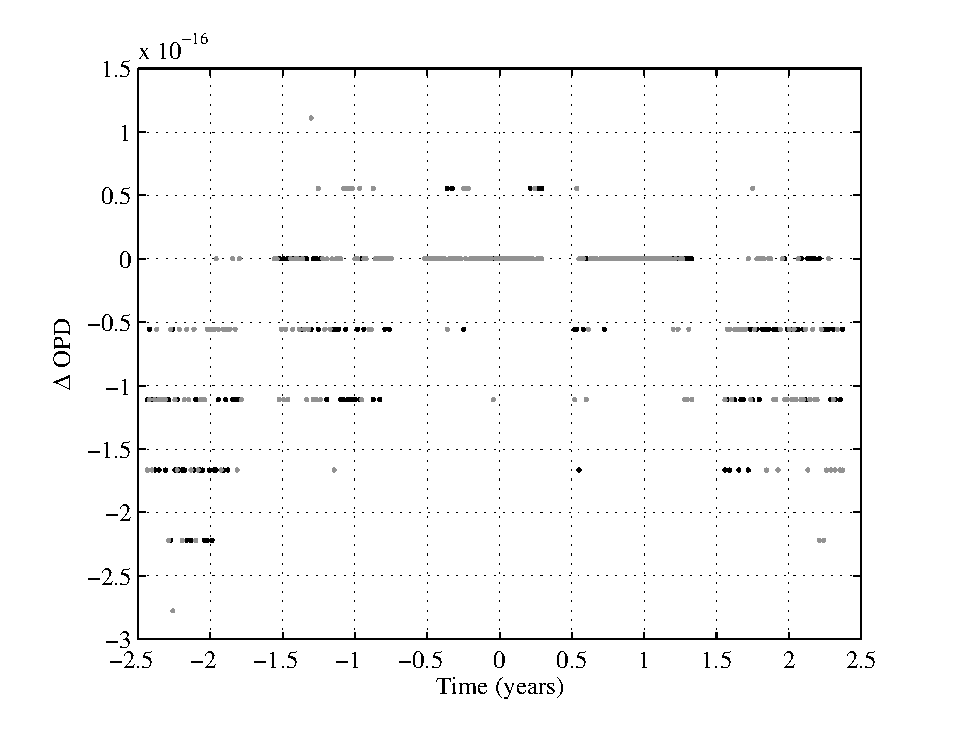
\includegraphics[width=5.5in]{./figures/apri_expansion}
 \caption[Second order expansion of astrometric observation equation assuming prior knowledge]{Difference between differential OPDs (between a sun-twin star and fixed centroid) using the second order expansion of $\hat\R_{s/sc}$ from \refeq{eq:rhat_expand2} and the  expansion from \refeq{eq:rhat_expand_apri} with assumed errors in parallax and barycenter motion of 1 mas and 1 mas/year, respectively.  The pattern in the residuals is due to the precision of the numerical data type used. The two curves represent the measurements along two orthogonal interferometer baseline orientations. \label{fig:apri_expansion}}
\end{figure} 
The difference between this equation and the OPD using the exact  expression for  $\hat\R_{s/sc}$ is almost exactly the same as for the second order expansion assuming no prior knowledge.  However, unlike \refeq{eq:rhat_expand2}, this equation is linear in the quantities to be estimated, thereby simplifying the filtering task.   In fact, the difference between differential OPDs calculated using Equations (\ref{eq:rhat_expand2}) and (\ref{eq:rhat_expand_apri}) is actually at the level of the numerical precision of the data type used in these simulations, which is what produces the characteristic residual pattern in \reffig{fig:apri_expansion}.  This figure highlights a very important point:  due to the small magnitudes of many of the quantities utilized in this analysis the limitations of the specific numerical representation become a real concern when constructing simulations.  Any computer generated value will have an associated finite precision, but specific representation schemas may actually introduce precision differences as functions of value magnitude.  For example, in MATLAB, the default numerical data type is a double precision, floating point number, encoded as:
\begin{equation}
2^e\times s
\end{equation}
where $e$ is the exponent and $s$ is the significand.  These are stored as 11 bits and 53 bits, respectively, as per the IEEE 754 standard \citep{IEEE2008}.  Because the exponent and significand are encoded with a finite number of bits, the minimum step size to the next available value in this schema is a function of the  current value.  Thus, differences between pairs of values of different orders will have different precisions \citep{moler2004numerical}.  For example, when encoding values of order 1 as double precision floats, the minimum step size to the next available value is on the order of 1$\times10^{-16}$.  However, when encoding values of order 1e6 (like, for example, the value of 10 pc in AU), the step size to the next available value is of order 1$\times10^{-10}$.

The particulars of the encoding become important when one wants to generate `ground truth' data, using, for example, the exact representation of the astrometric observation in \refeq{eq:rhat_ssc}.  In this case, certain values, such as $\R_s(t_0)$ are multiple orders of magnitude greater than 1, whereas the final result is many orders of magnitude less.  This means that numerical noise at the level of the desired signal could inadvertently be introduced into the simulated data.  In the simulations presented here, this only became significant when converting $\R_{s/sc}$ to a unit vector. One solution (the one employed here) is to generate the large values with an arbitrary precision data type using the appropriate number of digits.  Once the spacecraft to star unit vector is generated, all values are of sufficiently low order that the default fixed precision data type is sufficient for the remaining calculations.  To do so, it is necessary to use an arbitrary-precision data type, which simply encodes values using variable length significands, rather than the fixed bit scheme described above.  For the simulations here, sufficient precision was achieved by using the GNU multiple precision library (\url{http://gmplib.org/}), with the significand stored as 256 bits.  The numerical effect is quite limited in the simulations above (with the target star at 10 pc), but becomes much more pronounced for targets at 100 pc.  Figure \ref{fig:precision_test} shows the difference between differential OPDs using \refeq{eq:rhat_ssc}, with one simulation done using the default double precision data type for all values, and the other using the multiple precision data type.  The error between the two is close to 1$\times10^{-8}$ in magnitude, making it a significant noise contribution.
 \begin{figure}[ht]
\centering
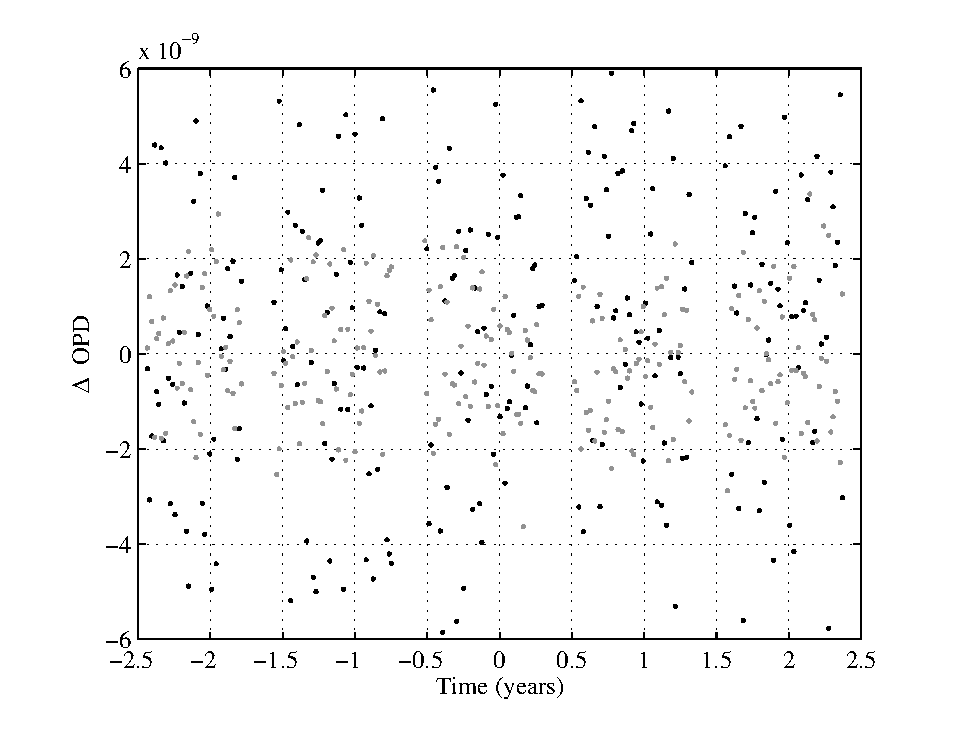
\includegraphics[width=5.5in]{./figures/precision_test}
 \caption[Numerical encoding precision test]{Difference between differential OPDs (between a sun-twin star and fixed centroid) using the exact formulation of $\hat\R_{s/sc}$ from \refeq{eq:rhat_ssc} with the default double precision data type and a multiple precision data type at 256 bits.  All values are the same as in previous simulations, except that the target star is placed at 100 pc. The two curves represent the measurements along two orthogonal interferometer baseline orientations. \label{fig:precision_test}}
\end{figure} 
%
%\begin{fleqn}
\begin{figure*}[ht]
\begin{equation}\label{eq:rhat_expand3}
\begin{split}
\hat\R_{s/sc} &\cdot \mf b_i \approx
\left\{\bar\R_{\mu0} + \delta\bar\R_\mu - \frac{1}{2} \bar\R_{\mu0} (\bar\R_{\mu0} \cdot \bar\R_{\mu0}) - \bar\R_{\mu0} (\hat\R_s(t_0) \cdot \bar\R_{\mu0})\right.\\
& {} - \delta\bar\R_\mu (\hat\R_s(t_0) \cdot \bar\R_{\mu0}) + \frac{3}{2} \bar\R_{\mu0} (\hat\R_s(t_0) \cdot \bar\R_{\mu0})^2 - \bar\R_{\mu0} (\hat\R_s(t_0) \cdot \delta\bar\R_\mu) \\ 
%
&{} + \left[\vphantom{\frac{1}{2}}\Delta \tilde\R_{s/G} - \tilde\R_{sc} +\left(\tilde\R_{sc} -  \Delta \tilde\R_{s/G}\right) (\hat\R_s(t_0) \cdot \bar\R_{\mu0}) \right.\\
&\left.{} + \bar\R_{\mu0}\left((\hat\R_s(t_0) \cdot \tilde\R_{sc}) -(\hat\R_s(t_0) \cdot \Delta \tilde\R_{s/G})\right)\vphantom{\frac{1}{2}}\right] \delta\varpi\\ 
%
&{} + 2\left[\vphantom{\frac{1}{2}}\left(\tilde\R_{sc}  -\Delta \tilde\R_{s/G}\right) (\hat\R_s(t_0) \cdot \Delta \tilde\R_{s/G})\right.\\
&\left.{}  + \left(\Delta \tilde\R_{s/G} - \tilde\R_{sc}\right)(\hat\R_s(t_0) \cdot \tilde\R_{sc})\vphantom{\frac{1}{2}}\right]\varpi_0\delta\varpi\\
%
&{} + \left[\Delta \tilde\R_{s/G} - \tilde\R_{sc} + \frac{1}{2}\left(\tilde\R_{sc} -\Delta \tilde\R_{s/G}\right) (\bar\R_{\mu0} \cdot \bar\R_{\mu0}) \right.\\
&{}+ \frac{3}{2} \left(\Delta \tilde\R_{s/G} -  \tilde\R_{sc} \right)(\hat\R_s(t_0) \cdot \bar\R_{\mu0})^2   + \bar\R_{\mu0} \left((\bar\R_{\mu0}\cdot \tilde\R_{sc}) -  (\bar\R_{\mu0} \cdot \Delta \tilde\R_{s/G})\right) \\
&{}     + \left(\tilde\R_{sc} - \Delta \tilde\R_{s/G}\right)\left((\hat\R_s(t_0) \cdot \bar\R_{\mu0}) + (\hat\R_s(t_0) \cdot \delta\bar\R_\mu)\right) \\
&{}+ \left(\bar\R_{\mu0} + \delta\bar\R_\mu\right)\left( (\hat\R_s(t_0) \cdot \tilde\R_{sc}) - (\hat\R_s(t_0) \cdot \Delta \tilde\R_{s/G}) \right)\\
&\left.{} + 3\bar\R_{\mu0} (\hat\R_s(t_0) \cdot \bar\R_{\mu0})\left( (\hat\R_s(t_0) \cdot \Delta \tilde\R_{s/G})  - (\hat\R_s(t_0) \cdot \tilde\R_{sc})\right)\vphantom{\frac{1}{2}}\right]\varpi_0\\
%
&{} + \left[\vphantom{\frac{1}{2}} \left(\tilde\R_{sc} -\Delta \tilde\R_{s/G}\right) (\bar\R_{\mu0} \cdot \Delta \tilde\R_{s/G}) + \left(\Delta \tilde\R_{s/G} -   \tilde\R_{sc}\right)(\bar\R_{\mu0}\cdot \tilde\R_{sc})\right.\\
&{} + \bar\R_{\mu0} (\Delta \tilde\R_{s/G} \cdot \tilde\R_{sc}) - \frac{1}{2} \bar\R_{\mu0}\left( (\Delta \tilde\R_{s/G} \cdot \Delta \tilde\R_{s/G}) + (\tilde\R_{sc} \cdot \tilde\R_{sc})\right)\\
&{}+ \left(\tilde\R_{sc}  - \Delta \tilde\R_{s/G}\right)\left( (\hat\R_s(t_0) \cdot \Delta \tilde\R_{s/G}) - (\hat\R_s(t_0) \cdot \tilde\R_{sc})\right) \\
&{} + 3\left(\Delta \tilde\R_{s/G} (\hat\R_s(t_0) \cdot \bar\R_{\mu0})  - \tilde\R_{sc} (\hat\R_s(t_0) \cdot \bar\R_{\mu0})\right)(\hat\R_s(t_0) \cdot \Delta \tilde\R_{s/G})\\
&{}+ 3\left(\tilde\R_{sc} - \Delta \tilde\R_{s/G}\right)(\hat\R_s(t_0) \cdot \bar\R_{\mu0}) (\hat\R_s(t_0) \cdot \tilde\R_{sc})  \\
&{} - 3\bar\R_{\mu0} (\hat\R_s(t_0) \cdot \Delta \tilde\R_{s/G}) (\hat\R_s(t_0) \cdot \tilde\R_{sc})\\
&\left.{} + \frac{3}{2} \bar\R_{\mu0}\left( (\hat\R_s(t_0) \cdot \Delta \tilde\R_{s/G})^2+ (\hat\R_s(t_0) \cdot \tilde\R_{sc})^2\right)\right]\varpi_0^2\\
%
&{} + \left[\left(\Delta \tilde\R_{s/G}  - \tilde\R_{sc}\right)(\Delta \tilde\R_{s/G} \cdot \tilde\R_{sc}) - \frac{1}{2}\left( \Delta \tilde\R_{s/G} +\tilde\R_{sc}\right)(\Delta \tilde\R_{s/G} \cdot \Delta \tilde\R_{s/G}) \right.\\
&{}+ \frac{1}{2} \left(\tilde\R_{sc} -  \Delta \tilde\R_{s/G} \right)(\tilde\R_{sc} \cdot \tilde\R_{sc}) + \frac{3}{2} \left(\Delta \tilde\R_{s/G}  - \tilde\R_{sc}\right)(\hat\R_s(t_0) \cdot \Delta \tilde\R_{s/G})^2 \\
&{} + 3\left(\tilde\R_{sc}- \Delta \tilde\R_{s/G}\right) (\hat\R_s(t_0) \cdot \Delta \tilde\R_{s/G}) (\hat\R_s(t_0) \cdot \tilde\R_{sc}) \\
&\left.\left.{} + \frac{3}{2} \left(\Delta \tilde\R_{s/G} - \tilde\R_{sc}\right) (\hat\R_s(t_0) \cdot \tilde\R_{sc})^2 \right]\varpi_0^3\right\}\cdot \mf b_i
\end{split}
\end{equation}
%\end{fleqn}
\end{figure*}

An alternative to this approach would be to use \refeq{eq:rhat_norm}.  All terms in this formulation (which is equivalent to \refeq{eq:rhat_ssc}) are of order 1 or less, so that the default double precision data type should be sufficient.  Unfortunately, use of this equation can also introduce numerical noise, if one is not careful in how the various terms are defined.  Terms such as $\R_\mu$ are essentially small values divided by very large values.  If they are not exactly defined, but rather calculated in software, then they will have the same problems as shown above.  Since this discussion applies only to the simulation or generated data, it is relatively simple to just assume values for barycenter motions that will give exact fractional values when scaled by the parallax, eliminating such concerns.  If we wished to update our expansions such that the residual was below the precision of the default double precision data type, we would need to retain terms proportional to $\varpi^3$.  However, in the case of the expansions assuming prior knowledge of parallax and barycenter motion, no higher order terms in $\delta \varpi$ would be needed, as seen in \refeq{eq:rhat_expand3}.

One assumption made in this analysis is that the error is of the same magnitude for all three components of $\bar\R_{\mu}$.  However, this ignores the fact that currently existing estimates for the first two components (the transverse motion) are derived from different sources than estimates for the third component (the radial motion).  While proper motions have been measured by space-based astrometric instruments, radial velocities are generally provided by ground-based doppler spectroscopy, and are inherently less accurate.  To address this, we can modify \refeq{eq:rhat_expand_apri} by separating $\delta\bar\R_\mu$ into two separate errors so that:
\begin{equation}\label{eq:rmu_redef}
\bar\R_{\mu} =  \bar\R_{\mu0}  +\delta\R_{R} + \delta\R_{T} 
\end{equation}
where $\delta\R_{R}$ and $\delta\R_{T}$ are due to errors in our prior knowledge of $V_R$ and $\mf V_T$, as defined in \refeq{eq:veldef}.

 We can now repeat the expansion performed to generate \refeq{eq:rhat_expand_apri}), substituting the right-hand side of \refeq{eq:rmu_redef} for $\bar\R_{\mu}$. The rules for keeping terms containing $ \delta\R_{T}$ remain the same as those for $\delta\bar\R_\mu$.  If we assume that $\delta\R_{R}$ is less than three orders of magnitude higher than $\delta\R_{T}$ (i.e., m/s radial velocity precision), then the expansion in \refeq{eq:rhat_expand_apri} must also retain terms proportional to  $\Vert \delta\R_{R} \Vert^n$ for $n <= 2$.  The result is that only one term, equal to $-\delta\R_{R}( \hat\R_s(t_0) \cdot  \delta\R_{R}) = -\delta\R_{R}\Vert\delta\R_R\Vert$, must be added to \refeq{eq:rhat_expand_apri} to account for the lower precision of the prior radial velocity measurement.

\section{Applications}\label{sec:filterApplications}
In this section we will explore some applications of the formalism built up throughout the chapter.  In particular, we will discuss how to construct a filter to combine multiple observations of one planetary system, and examine whether the filtering framework can help to resolve confusion in the imaging of multi-planet systems.  Because of the inherent synergies between doppler spectroscopy and astrometry (one essentially measures the projected component least observable by the other), there has always been significant interest in combining the two \citep{sozzetti2005}.  One commonly proposed method of combining these data sets (or just the two signal channels produced by astrometry) is the formulation of a joint periodogram \citep{catanzarite2006}, which is just a summation of independent Lomb-Scargle periodograms.  This approach has the drawback of ignoring much of the known dynamics of orbital motion.  In particular, as both eccentricity and projection effects cause deviations from pure harmonic motion in the observations, they are only separable by performing full orbital fits to the significant periodicities found by the periodogram, which themselves will deviate from the true periods due to these same effects.

When there are significant n-body effects, the periodogram has the effect of averaging over any variations in orbital periods, which can lead to Keplerian fits that do not actually correspond to the best-fit orbit at any specific time in the data set.  We can demonstrate this by simulating a system with two Jupiter-mass planets with initial conditions corresponding to a 1:3 mean motion resonance.  As the initial conditions do not describe a stable resonance, the orbits do not maintain an exact 1:3 period ratio, but do exhibit significant deviations from the equivalent mean Keplerian fits, as demonstrated in \reffig{fig:twoJupSystem}.  Without any added noise, the Lomb-Scargle periodogram has no trouble pulling out two significant periodicities (\reffig{fig:twoJupPeriodogram}) corresponding to the two planets using just one component of the star's velocity.  However, if we compare the periods derived from the periodogram with the osculating periods, we immediately see the averaging effect described above (\reffig{fig:twoJupOscPer}).
\begin{figure}[ht]
\centering
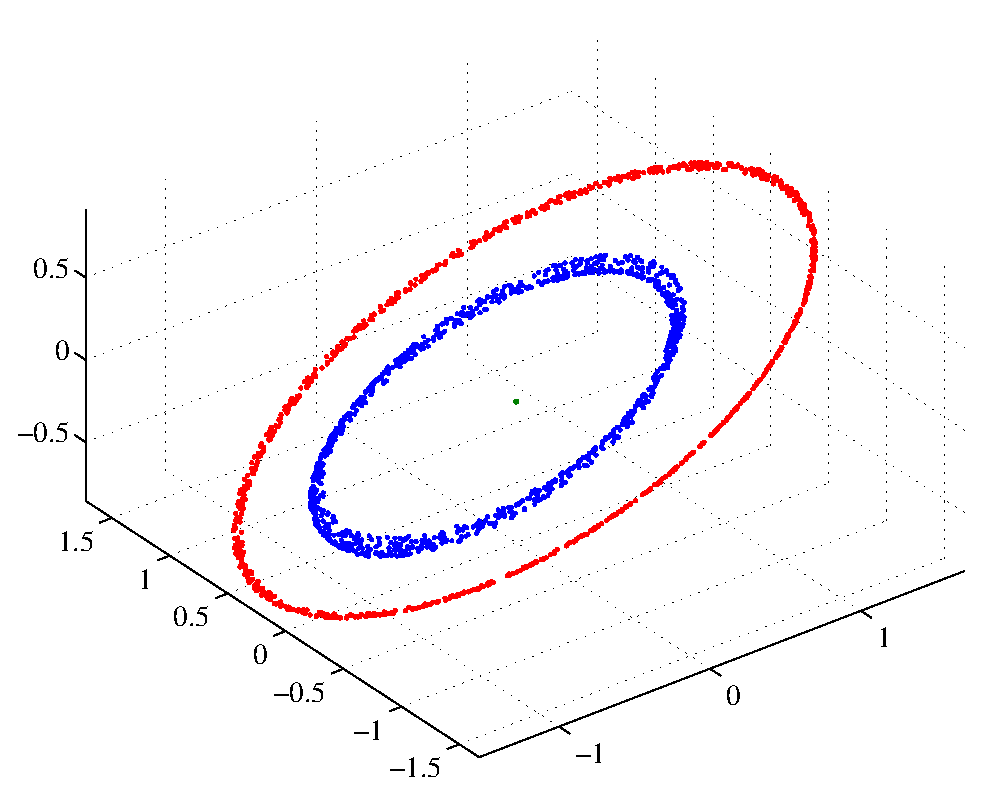
\includegraphics[width=5.5in]{./figures/twoJupSystem}
 \caption[Two Jupiter system]{Integration of a system composed of a sun-twin and two Jupiters for 75 orbits of the innermost planet. \label{fig:twoJupSystem}}
\end{figure} 
\begin{figure}[ht]
\centering
\subfigure[]{
\includegraphics[height=2.25in]{./figures/twoJupPeriodogram}\label{fig:twoJupPeriodogram}}
\subfigure[]{
\includegraphics[height=2.25in]{./figures/twoJupOscPer}\label{fig:twoJupOscPer}}
 \caption[Two Jupiter system periods]{(a) Lomb-Scargle periodogram of $\hat z$-axis component of star velocity for system from \reffig{fig:twoJupSystem}. The red ticks represent the significant frequencies. (b) The orbital period of the Keplerian orbital fit for every time step for the outer planet (blue) and the period from the periodogram (red).}
\end{figure}

What's particularly interesting about this system is that the osculating arguments or periapsis for both planets remain very stable in time (within 5\% of the initial value for the inner planet and within 7\% of the initial value for the outer planet), and the rest of the orbital elements osculate on time frames longer than one orbit.  This indicates that the instantaneous Keplerian fits do describe meaningful orbits (unlike the case of true resonances where elements osculate on time scales faster than a single orbital period), and information is being discarded by averaging over the entire data set.  In the next section we will see how the filtering formalism allows us to fit the dynamic orbits, rather than average Keplerian elements.

\subsection{Combined Astrometry and Doppler Spectroscopy}
To test the filter's ability to fit orbits we use the same type of simulated data as shown in the previous section, except with added astrometric effects and instrument noise. We begin with a single planet of 1 M$_\oplus$ on an Earth-like orbit (1 AU semi-major axis, but arbitrarily oriented with respect to the instrument line of sight) and simulate the stellar reflex.  To simulate the data set that would be produced by an astrometric space-based observatory, we take snapshots of the stellar reflex over a 15 year period, with the first 10 years composed solely of doppler spectroscopy data, and the final 5 years containing a mix of radial velocity and astrometric measurements.  The doppler spectroscopy data is assumed to cover a longer period since it can be taken using a ground-based observatory, whereas the assumed precision of the astrometry requires a space-based instrument.  The noise variance applied to the data has a magnitude of 0.82 $\mu$as for the astrometric data and 1 m/s for the doppler spectroscopy data, as shown in \reffig{fig:astrom_dat}.
\begin{figure}[ht]
\centering
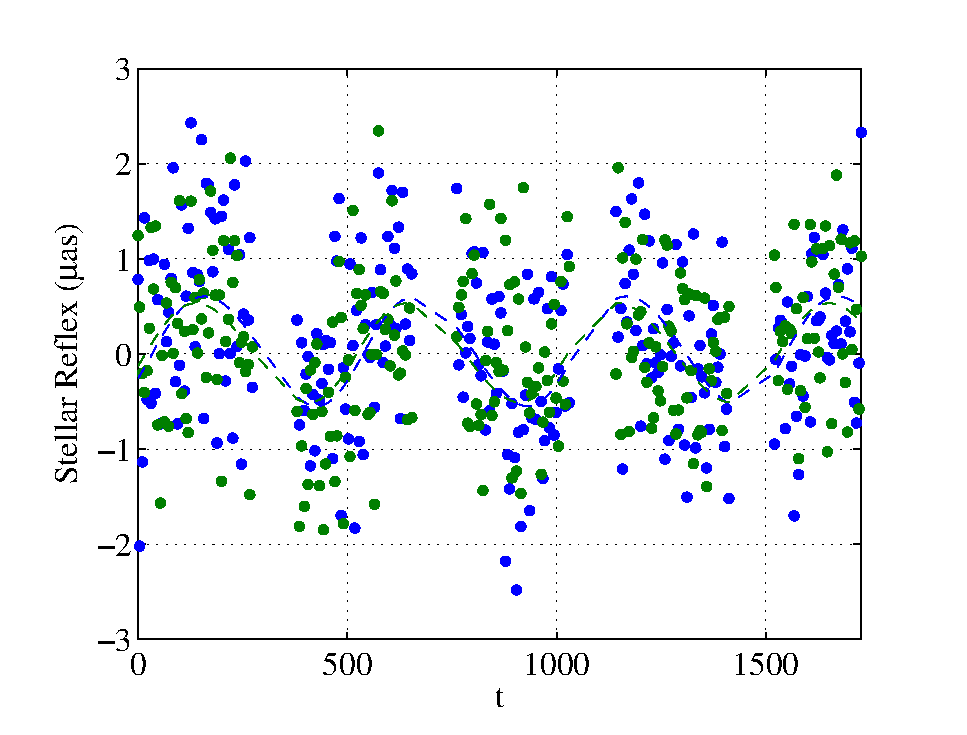
\includegraphics[width=5in]{./figures/astrom_dat}
 \caption[Astrometric observation noise]{Two channels (orthogonal instrument baselines) of a simulated astrometric observation of an Earth-mass planet.  The dashed lines represent the true signal, whereas the points are the noisy (0.82 $\mu$as variance) measurement. \label{fig:astrom_dat}}
\end{figure} 

\begin{figure}[ht]
 \begin{center}
  \subfigure[Position]{
   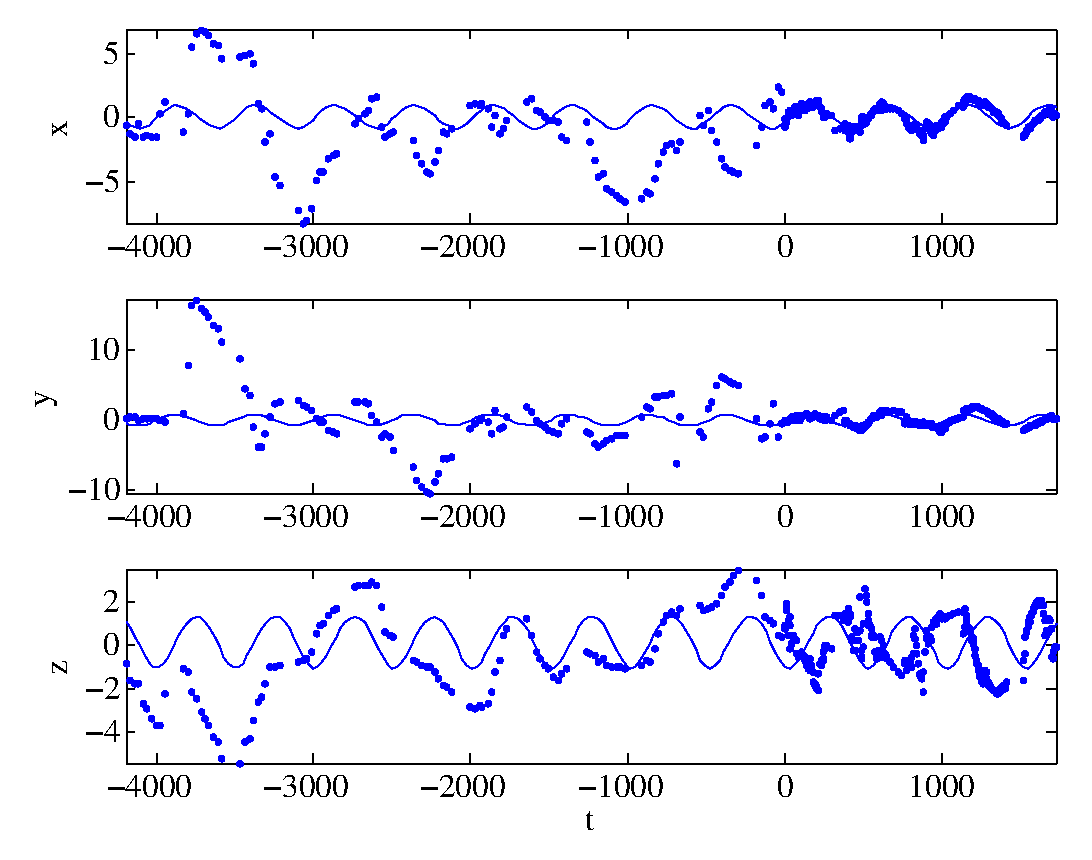
\includegraphics[width=2.9in,clip=true,trim=0.1in 0in 0.1in 0in]{./figures/true_mass2_pos}}
   \subfigure[Velocity]{\includegraphics[width=2.9in,clip=true,trim=0.1in 0in 0.1in 0in]{./figures/true_mass2_vel}}
 \end{center}
 \caption[Filtered results for Earth mass planet]{ \label{fig:true_mass_rv}
	Filter outputs of planet position and velocity, plotted as points over solid lines representing the true positions for a single Earth-mass planet system.}
\end{figure}
\reffig{fig:true_mass_rv} shows the output of the hybrid, constrained EKF for the case of the single Earth-mass planet.  The plots represent the estimates of the position and velocity (in AU and AU/day, respectively) plotted in components in the tangent frame.  The time is in days, with the zero epoch coinciding with the first astrometric measurement (i.e., estimates at times $t < 0$ are based solely on radial velocity measurements). We can immediately see that the filter performs quite well, despite the very large noise level, except for expected errors in badly observed components.  The state is initialized with the planet mass set to its correct value, but with randomized initial positions and velocities (consistent with the observations and a closed (negative Keplerian energy) orbit).  The initial proper motion and parallax have errors of 1 mas/year and 1 mas, respectively.  Although the system does not have true process noise, a diagonal $\mf Q$ with values six orders of magnitude below the state estimate is introduced in order to keep the filter from falling into local minima.  Initial states are also propagated via one UKF step to more closely model the state distribution, while initial covariances are produced via Monte Carlo simulation, as in \reffig{fig:covarianceEstimate}.

\reffig{fig:true_mass_err} displays the same data as errors (true state minus the estimate), along with the variance estimated by the filter.  It is quite encouraging to see that the filter is doing a credible job of estimating how well it is doing almost everywhere in the data set. There are, however, large spikes in  the velocity error estimate after the astrometric data kicks in.  These are due to numerical effects in the current state prediction integration, and are removed in subsequent smoothing runs.
\begin{figure}[ht]
 \begin{center}
 \subfigure[Position Error]{
   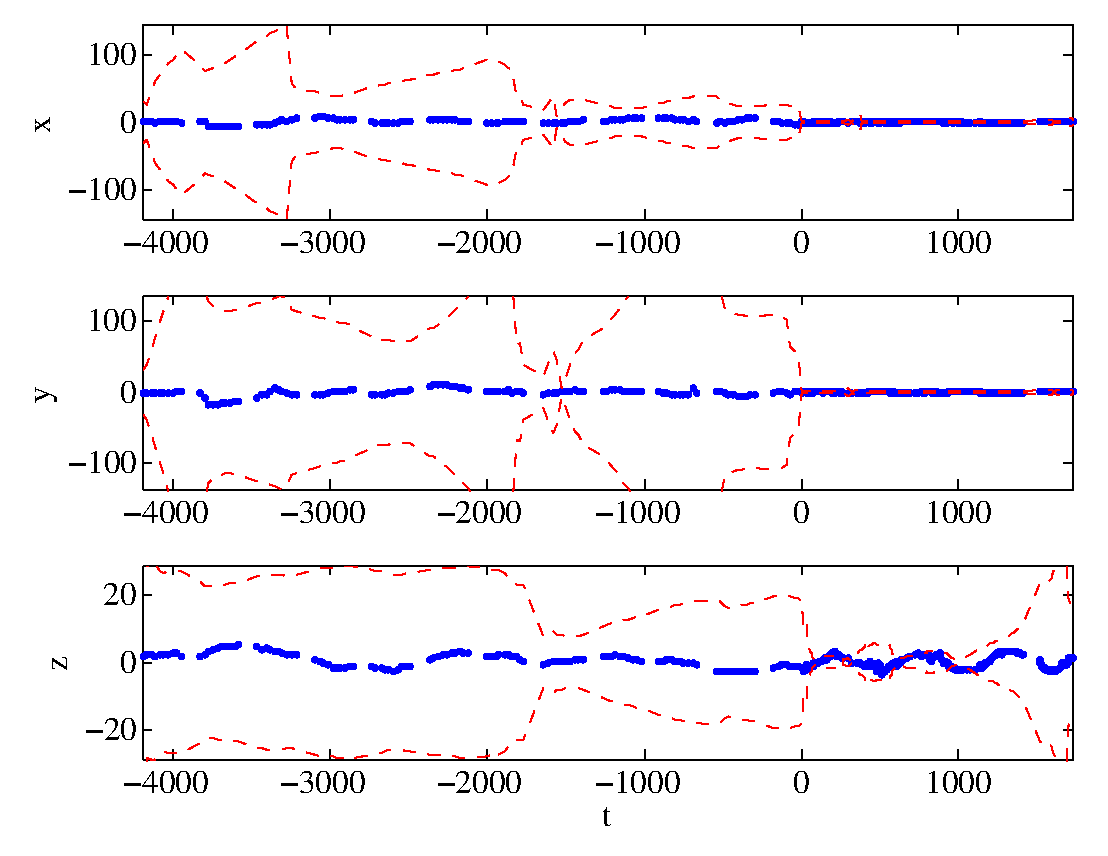
\includegraphics[width=2.9in,clip=true,trim=0.1in 0in 0.1in 0in]{./figures/true_mass2_pos_err}}
   \subfigure[Velocity Error]{
    \includegraphics[width=2.9in,clip=true,trim=0.1in 0in 0.1in 0in]{./figures/true_mass2_vel_err}}
 \end{center}
 \caption[Filter estimated error for Earth mass planet]{ \label{fig:true_mass_err}
	Error of state estimate in  position and velocity plotted as points with the filter's variance estimate plotted as dashed lines for data in \reffig{fig:true_mass_rv}.}
\end{figure}

We can also study the effects of varying the initial mass estimate.  Through a large number of simulations, it is found that the filter generally fails to converge for the entire data set when the assumed mass of the planet is more than 50\% off from the true mass (in cases where convergence occurs, the described orbits are highly eccentric and do not correspond at all to the actual orbits).  Unfortunately, for assumed masses within 50\% of the true mass, the filter can actually converge to state estimates with covariances lower than that produced by the true mass.  In cases where the mass is within 50\% of the true mass, the constraints placed on the filter generally stop the mass estimate from diverging to any large extent from its initial value.  \reffig{fig:filtVar} shows the mean variances for position produced by the filter, as a function of error in the planetary mass.
\begin{figure}[ht]
 \begin{center}
   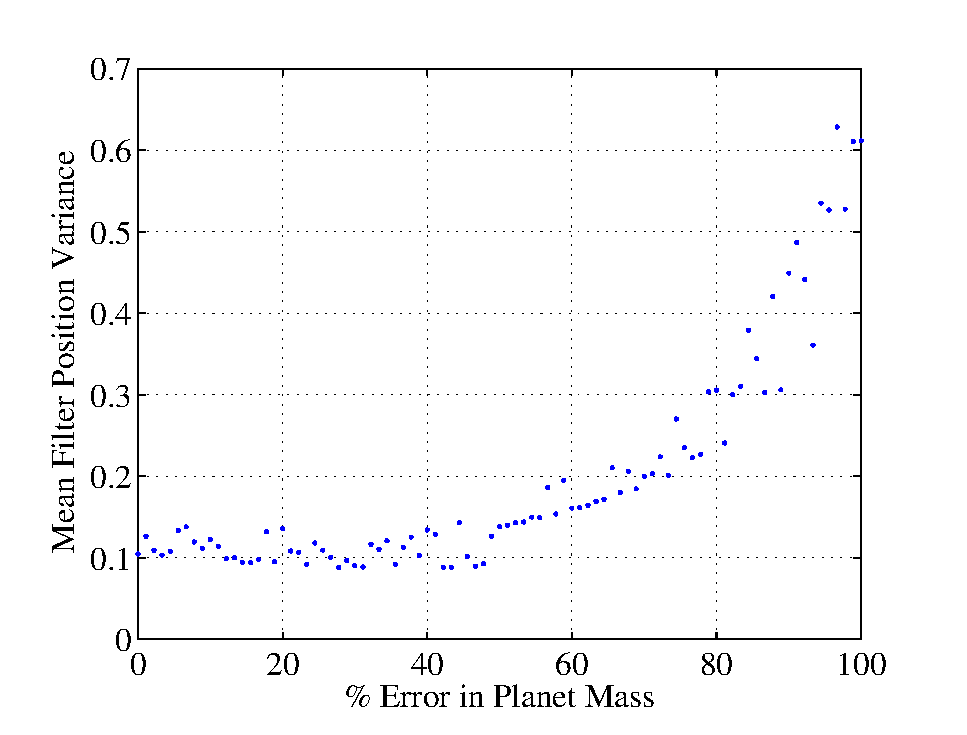
\includegraphics[width=4.5in,clip=true,trim=0.1in 0in 0.1in 0in]{./figures/filtVar_v_Err} 
 \end{center}
 \caption[Mean filter variance for increasing planet mass error]{ \label{fig:filtVar} Mean filter variance estimate plotted as a function of error in initial planet mass.}
\end{figure}

These results are very promising, most especially because of how well the filter does at estimating its own error.  The fact that the variance estimates bound the true error at all filter steps gives us great confidence in the filter's estimation of its performance.  Furthermore, the filter does an excellent job of tracking the more observable states (the sky plane positions and radial velocities) and at least captures the proper periodicities in the remaining state.  Unfortunately, the radial position estimate deviates at the end of the run, and the velocity states show signs of over-fitting to the observations.  The fact that the initial mass estimate has to be within 50\% of the true mass for the filter to perform well also indicates that this particular filter may be unsuitable for smaller planets with such low signal to noise values.  It is possible that a large-scale particle filter more capable of modeling the state distribution accurately would perform better.

Turning to the multi-planet case, we repeat the simulation, now including the Earth-mass planet and a Jupiter mass planet on a Jupiter-like orbit.   \reffig{fig:jup_mass_err} shows the filter estimate error for the Jupiter mass planet, which, as expected, is approximately a factor of 100 lower than that for the Earth-mass planet.  Because it dominates the astrometric signal to such a large extent, the filter has no problem estimating this planet's state.  Unfortunately, the Earth-mass signal becomes lost in this much larger one, and all states estimates have variances an order of magnitude higher than those produced in the case of the Earth-mass planet alone.
\begin{figure}[ht!]
 \begin{center}
  \subfigure[Position Error]{
   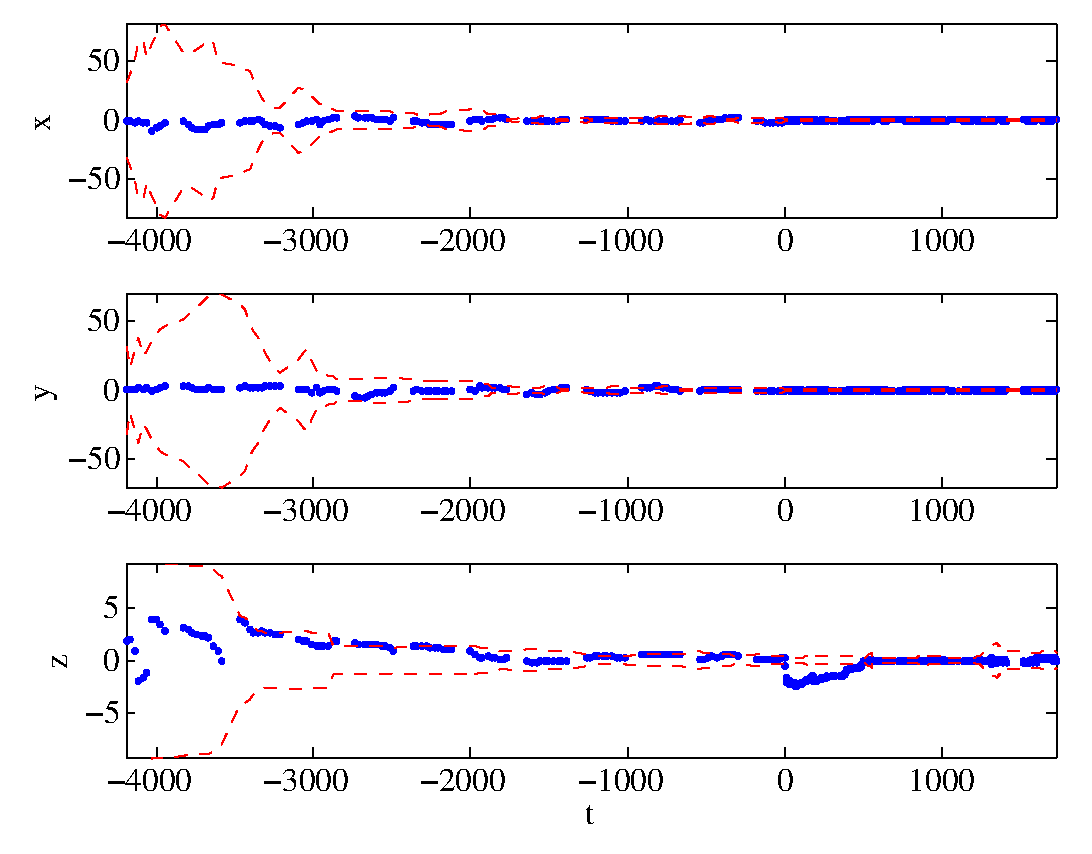
\includegraphics[width=2.9in,clip=true,trim=0.1in 0in 0.1in 0in]{./figures/jup_mass_pos_err}}
   \subfigure[Velocity Error]{
    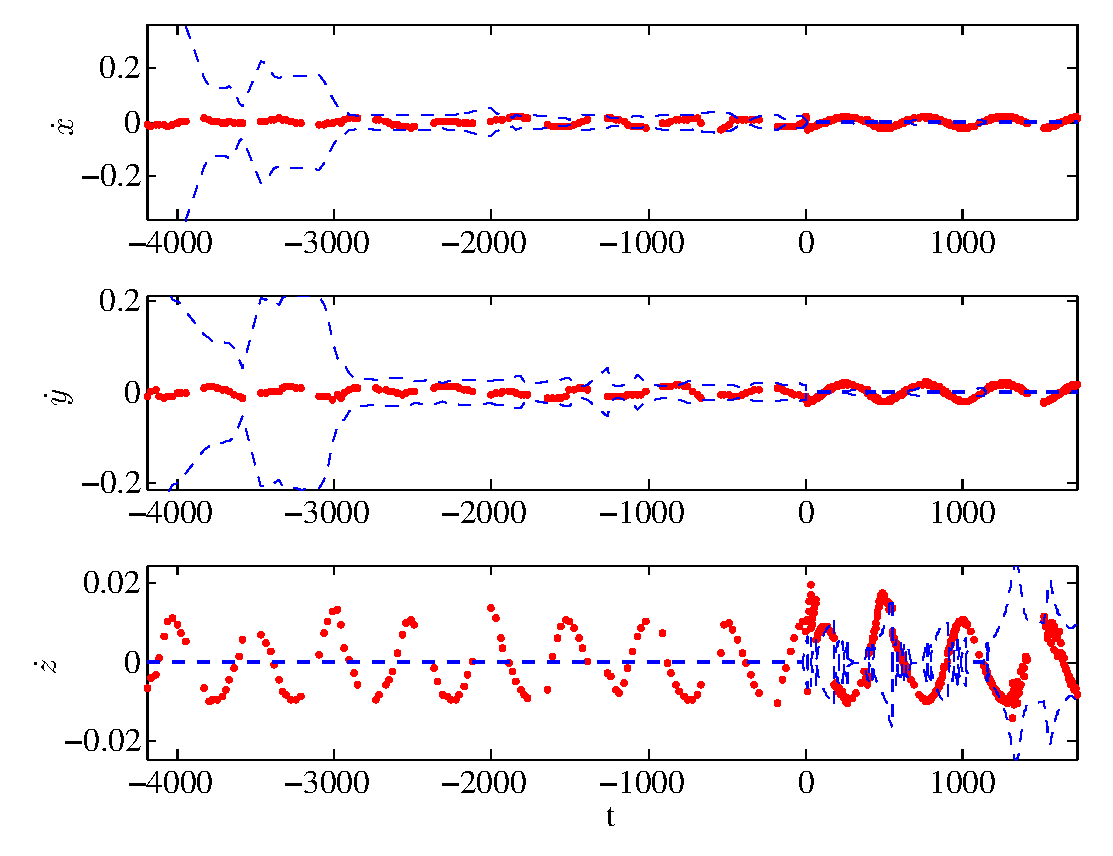
\includegraphics[width=2.9in,clip=true,trim=0.1in 0in 0.1in 0in]{./figures/jup_mass_vel_err}}
 \end{center}
 \caption[Filter estimated error for a Jupiter mass planet]{ \label{fig:jup_mass_err}
	Error of state estimate in  position and velocity plotted as points with the filter's variance estimate plotted as dashed lines for a Jupiter mass planet in multi-body system.}
\end{figure}

Due to the highly nonlinear observation functions and very high noise levels, the filter performance in terms of orbit fitting is relatively poor with this data set.  However, several important things are demonstrated by these simulations.  First, it is possible to swap out different observation functions at each time step without destabilizing the filter.  Second, we have demonstrated the capability to treat mass as one of the state parameters, as long as the initial mass estimate is sufficiently close to the true mass.  These estimates can be greatly constrained by using the periodogram analysis combined with the PDFs derived in \S\ref{sec:analytic_dists}. Finally, in cases where the filter does converge upon an orbit, it is tracking the actual positions and velocities of the planets, rather than averaged orbital elements, and can thus potentially tell us more about the exosystem than any Keplerian orbital fit.  More work, however, is required on creating a filter capable of dealing with both the nonlinearities of the dynamics and observation functions as well as the high level of noise in the observations. 

\subsection{Filter Applications for Direct Detection}

Following the simulation methodology adopted in the previous section, we can also consider what happens when long term doppler spectroscopy is  followed by one single successful direct detection.  In this case, we would like to also test whether imaging can help fit orbits in data sets where there is less than a whole orbital period of observations.  To do so, we simulate 5 years (approximately half of one orbit) of doppler spectroscopy measurements of a sun mass star with a a Jupiter mass planet, immediately followed by one image taken with an instrument identical to THEIA's XPC, with an assumed centroiding accuracy of one tenth of one pixel.

\begin{figure}[ht]
 \begin{center}
\subfigure[Planet Position]{\includegraphics[width=2.9in,clip=true,trim=0.6in 0in 0.1in 0in]{./figures/planpos1}}
 \subfigure[Planet Velocity]{\includegraphics[width=2.9in,clip=true,trim=0.6in 0in 0.1in 0in]{./figures/planvel1}}    
 \end{center}
 \caption[Filter output for RV]{Planet position and velocity components (solid lines) and filter output (points) for half of one period of doppler spectroscopy observations of a Jupiter mass planet.  Even with smoothing and multiple random re-initializations, the filter is unable to track the true state even approximately. \label{fig:filtOutRV}}
\end{figure}
\reffig{fig:filtOutRV} shows the filter output when using only the doppler spectroscopy data set.  Regardless of the initial conditions and the number of smoothing steps, the filter is unable to track the true state values.  It is interesting to note, however, that the instantaneous orbital elements produced by fitting Keplerian orbits to the filter state estimates do generate approximately correct orbital periods.

 \reffig{fig:filtOutRVdd} shows the results of filtering the same data set, but now adding one direct detection immediately after the last doppler spectroscopy measurement.  The direct detection immediately transfers the position state elements much nearer to their true values (with a larger error on the third component due to the nonlinearity in that observation).  The velocity states are still poorly estimated as they are not observed at all by the direct detection.

\begin{figure}[ht]
 \begin{center}
\subfigure[Planet Position]{\includegraphics[width=2.9in,clip=true,trim=0.6in 0in 0.1in 0in]{./figures/planpos2}}
 \subfigure[Planet Velocity]{\includegraphics[width=2.9in,clip=true,trim=0.6in 0in 0.1in 0in]{./figures/planvel2}}    
 \end{center}
 \caption[Filter output for RV and imaging]{Planet position and velocity components (solid lines) and filter output (points) for half of one period of doppler spectroscopy observations of a Jupiter mass planet and one direct detection.  The square marks represent the filter state after the inclusion of the direct detection. \label{fig:filtOutRVdd}}
  \end{figure}
  \begin{figure}[ht]
 \begin{center}
\subfigure[Planet Position]{\includegraphics[width=2.9in,clip=true,trim=0.6in 0in 0.1in 0in]{./figures/planpos3}}
 \subfigure[Planet Velocity]{\includegraphics[width=2.9in,clip=true,trim=0.6in 0in 0.1in 0in]{./figures/planvel3}}    
 \end{center}
 \caption[Filter and smoother output for RV and imaging]{Planet position and velocity components (solid lines) and filter output (points) for half of one period of doppler spectroscopy observations of a Jupiter mass planet and one direct detection with multiple filtering and smoothing steps. \label{fig:filtOutRVdd2}}
 \end{figure}
 
 Finally, \reffig{fig:filtOutRVdd2} repeats the simulation but adds two additional smoothing and filtering runs (i.e., running the entire data set forwards and backwards in time three times).  Both the positions and velocities are now much more closely constrained to the true states, although a negative consequence of the multiple smoothings is the over-fitting of the velocity state elements.  Because of this, the instantaneous orbital elements generated from the filter outputs can have very high errors, although the average orbital elements are very close (within 5\%) of their true values.

 \begin{figure}[ht]
 \begin{center}
    \includegraphics[width=4.5in]{./figures/estVariance}
 \end{center}
\caption[State variance estimates for confused data set]{Estimated variance of planet state (sum of covariance diagonal) for data sets composed of measurements of one planet (solid lines) and two different planets (dashed lines). \label{fig:estVars}}
\end{figure}

An alternate application for direct detection data returns to the question of possible confusion in multiple planet systems discussed in \S\ref{sec:scheduling}.  We can now evaluate what happens when data from observations of two different planets is filtered with a state assuming that they are observations of the same planet at different times.   Because stable orbits generally have to be sufficiently separated to remain stable, it is most likely that confusion will be due to projection effects from the inclination of the exosystem.  If we inadvertently create a data set composed of observations of two different planets, the filter will effectively be trying to estimate a state distribution composed of two separate distributions.  While these are not fully independent (due to n-body effects and the requirements of system stability), they will tend to make the filter's target distribution significantly bimodal.  This bimodality should, given enough filtering steps, cause the state element variance to increase.

To test this application, we again simulate our two Jupiter system, generating one data set with five observations of the outer planet, and another data set with ten observations split evenly between the two planets.  The system is highly inclined (70$^\circ$) so that the apparent separations of the two planets can be very similar.  \reffig{fig:estVars} shows the sum of the estimated variances (covariance diagonal elements) as a function of filter time step.  As predicted, the inclusion of a mixed state does not initially have a great effect on the covariance estimate, but with a sufficient number of observations, the variance in the state distribution becomes much more apparent.  These results indicate that the filtering framework can be a highly useful tool for validating data sets and picking out suspect observations.

\bigskip
\bigskip

The applications presented here represent just a tiny fraction of possible uses for the formalism developed in the first part of the chapter.  What's most important is the fact that because the very essence of the dynamic filter is the possibility of time-varying observation functions, this is the ideal tool for putting together complicated data sets with multiple information sources.  This framework also appears to be a good choice for tracking exosystem dynamics, although the inherent nonlinearities of these systems and observations, and the high measurement noises make this a very difficult task, and necessitate more work in filter development.